\documentclass[10pt]{beamer}
\usetheme[progressbar=frametitle]{metropolis}
\usepackage{appendixnumberbeamer}
\usepackage[T1]{fontenc}
\usepackage{booktabs}
\usepackage[scale=2]{ccicons}
\usepackage{adjustbox}
\usepackage{pgfplots}
\usepgfplotslibrary{dateplot}
\setbeamertemplate{footline}[frame number]
\usepackage{xspace}
\newcommand{\themename}{\textbf{\textsc{metropolis}}\xspace}

\title{Głębokie uczenie wielozadaniowe}
\subtitle{dla semantycznej analizy wnętrz}
\date{\today}
\date{}
\author{Piotr Hondra}
\institute{
    promotor: mgr inż. Maciej Stefańczyk \\
    kierunek: Automatyka i Robotytka \\
    Instytut Automatyki i Informatyki Stosowanej}
    \titlegraphic{\centering
\includegraphics[height=1cm]{images/eiti.pdf}}
    
    \begin{document}
    
    \maketitle
\begin{frame}{Cel pracy}

    \metroset{block=fill}
    \onslide+<2->
    \begin{block}{Cel pracy}
        Zbadanie problemu wspólnej segmentacji semantycznej i~klasyfikacji scen we wnętrzach.
    \end{block}

    
    \begin{itemize}
        \onslide+<3->\item Opracowanie architektury wielozadaniowej
        \onslide+<4->\item Przeprowadzenie łącznego uczenia
        \onslide+<5->\item Ewaluacja 
    \end{itemize}
    
\end{frame}

\begin{frame}{Segmentacja semantyczna oraz klasyfikacja sceny }
    \begin{figure}
        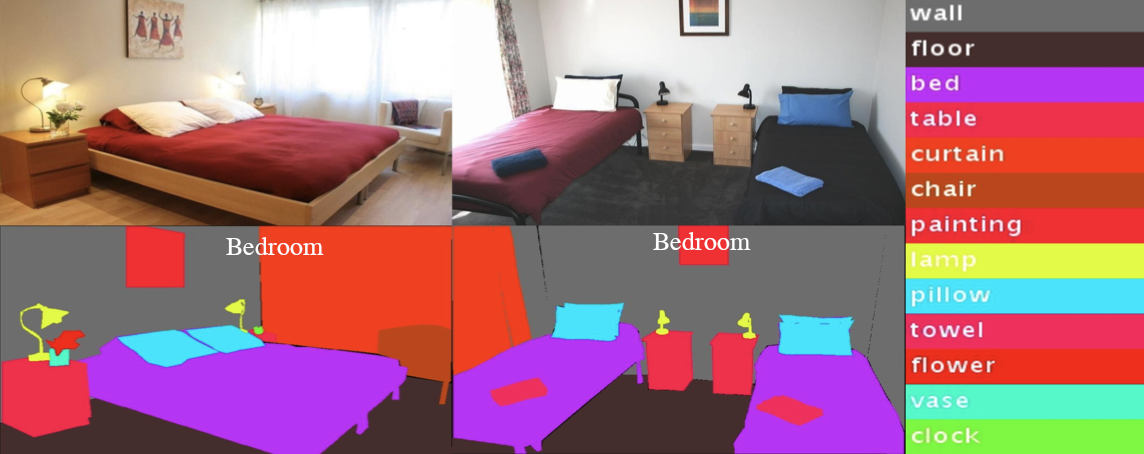
\includegraphics[height=0.5\textheight]{images/segment2.png}
        \caption{\cite{zhang2018context}.}
    \end{figure}
\end{frame}
\begin{frame}{Motywacje pracy}
    \begin{itemize}
        \item Robotyka
        \begin{itemize}
            \item nawigacja
            \item manipulacja obiektami
            \item interakcja człowiek-robot
        \end{itemize}
        \item Zarządzanie budynkiem
        \begin{itemize}
            \item zarządzanie energią
            \item bezpieczeństwo
        \end{itemize}
        \item Rozszerzona rzeczywistość
    \end{itemize}
\end{frame}

\section*{Zbiór danych}
\begin{frame}{Zbiór danych}
    \begin{figure}
        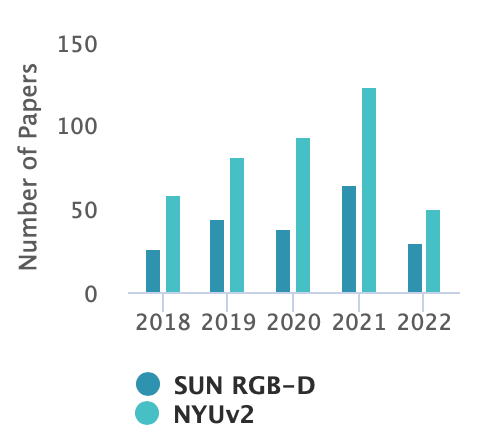
\includegraphics[height=0.7\textheight]{images/stats-dataset.png}
        \caption[]{Szacowana liczba cytowań w latach 2018-2022 \href{https://paperswithcode.com/dataset/sun-rgb-d}{[paperswithcode.com]}}
    \end{figure}
\end{frame}

\begin{frame}{Zbiór danych}
    \begin{columns}
        \begin{column}{0.5\textwidth}
            \begin{figure}
                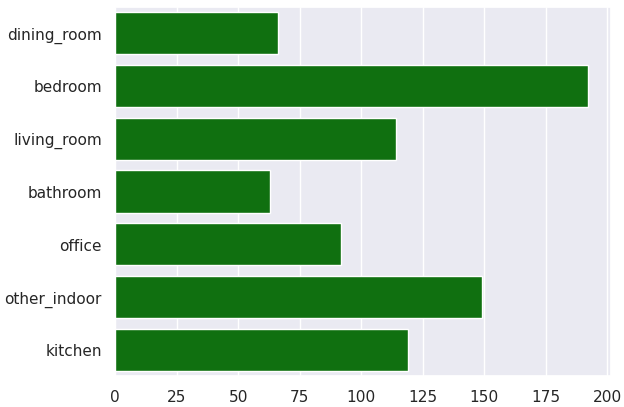
\includegraphics[width=\textwidth]{images/scene.png}
                \caption[]{Histogram klas dla zadania klasyfikacji sceny.}
            \end{figure}
            
        \end{column}

        \begin{column}{0.5\textwidth}
            
            \begin{figure}
                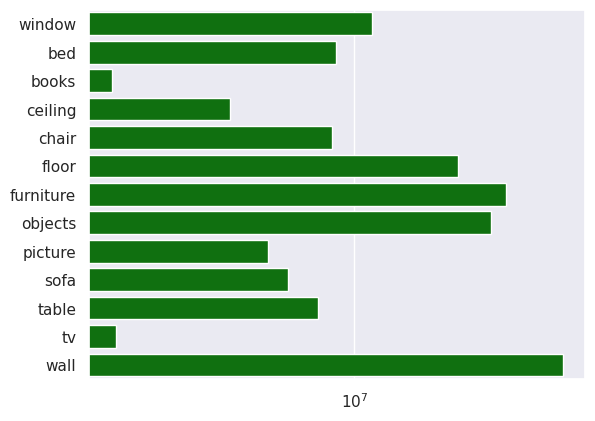
\includegraphics[width=\textwidth]{images/eda-seg13.png}
                \caption[]{Histogram pixeli klas dla zadania segmentacji semantycznej.}
            \end{figure}
        \end{column}
    \end{columns}
\end{frame}
\section*{Rozwiązanie problemu}
\begin{frame}{Rozwiązanie problemu - przedstawienie architektury}
    \begin{figure}
        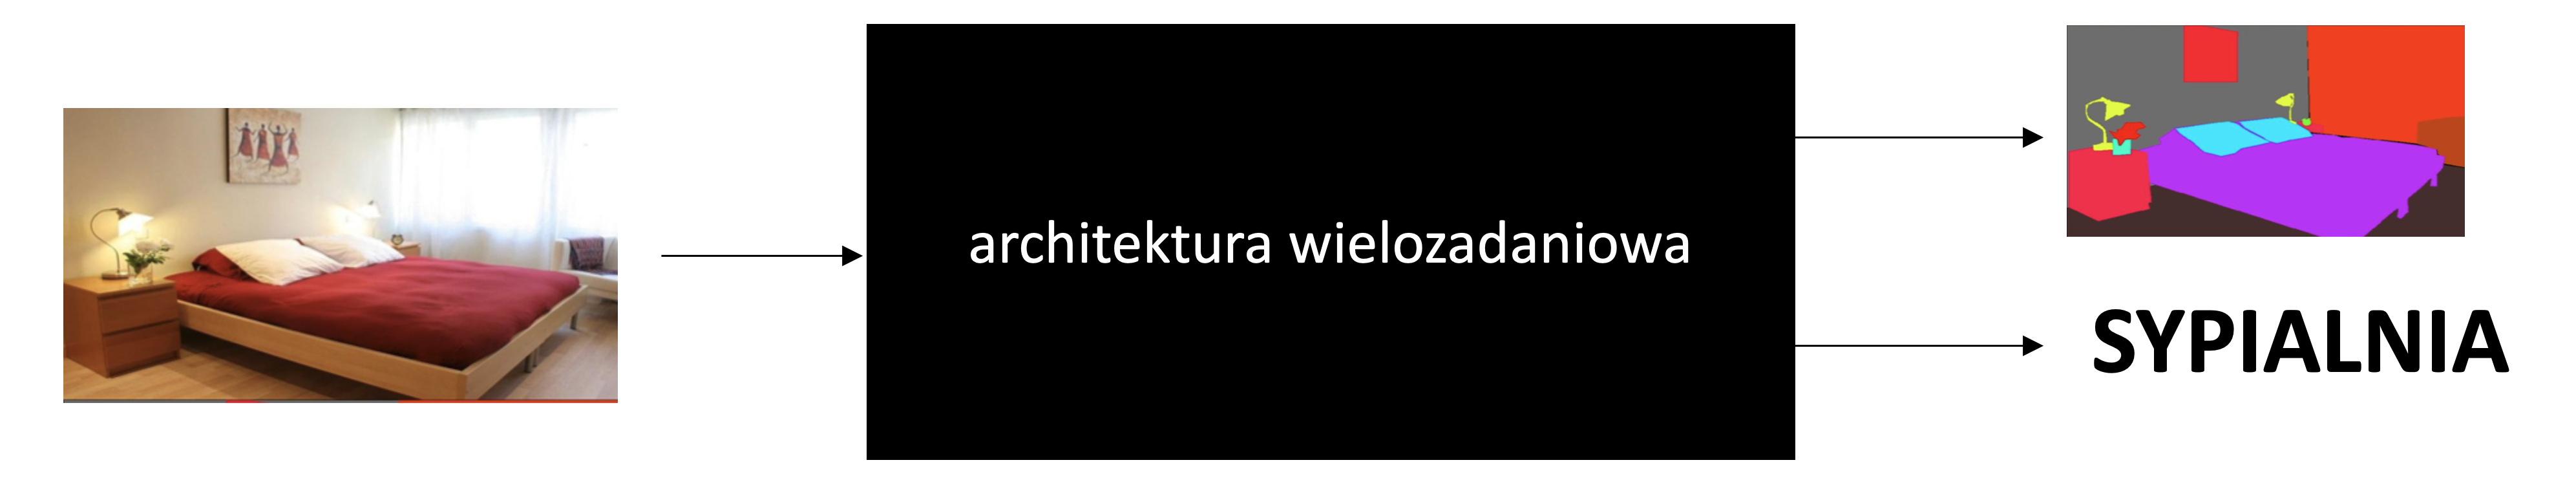
\includegraphics[width=\textwidth]{images/blackbox-2.png}
        \caption{Architektura sieci zastosowana w pracy inżynierskiej jako model czarnej skrzynki.}
    \end{figure}
\end{frame}


\section*{Opis eksperymentów}
\begin{frame}{Frame Title}
    \begin{columns}
        \begin{column}{0.5\textwidth}
            \begin{itemize}
               \item Uczenie wielozadaniowe
            \end{itemize}
        \end{column}

        \begin{column}{0.5\textwidth}
            \begin{figure}
                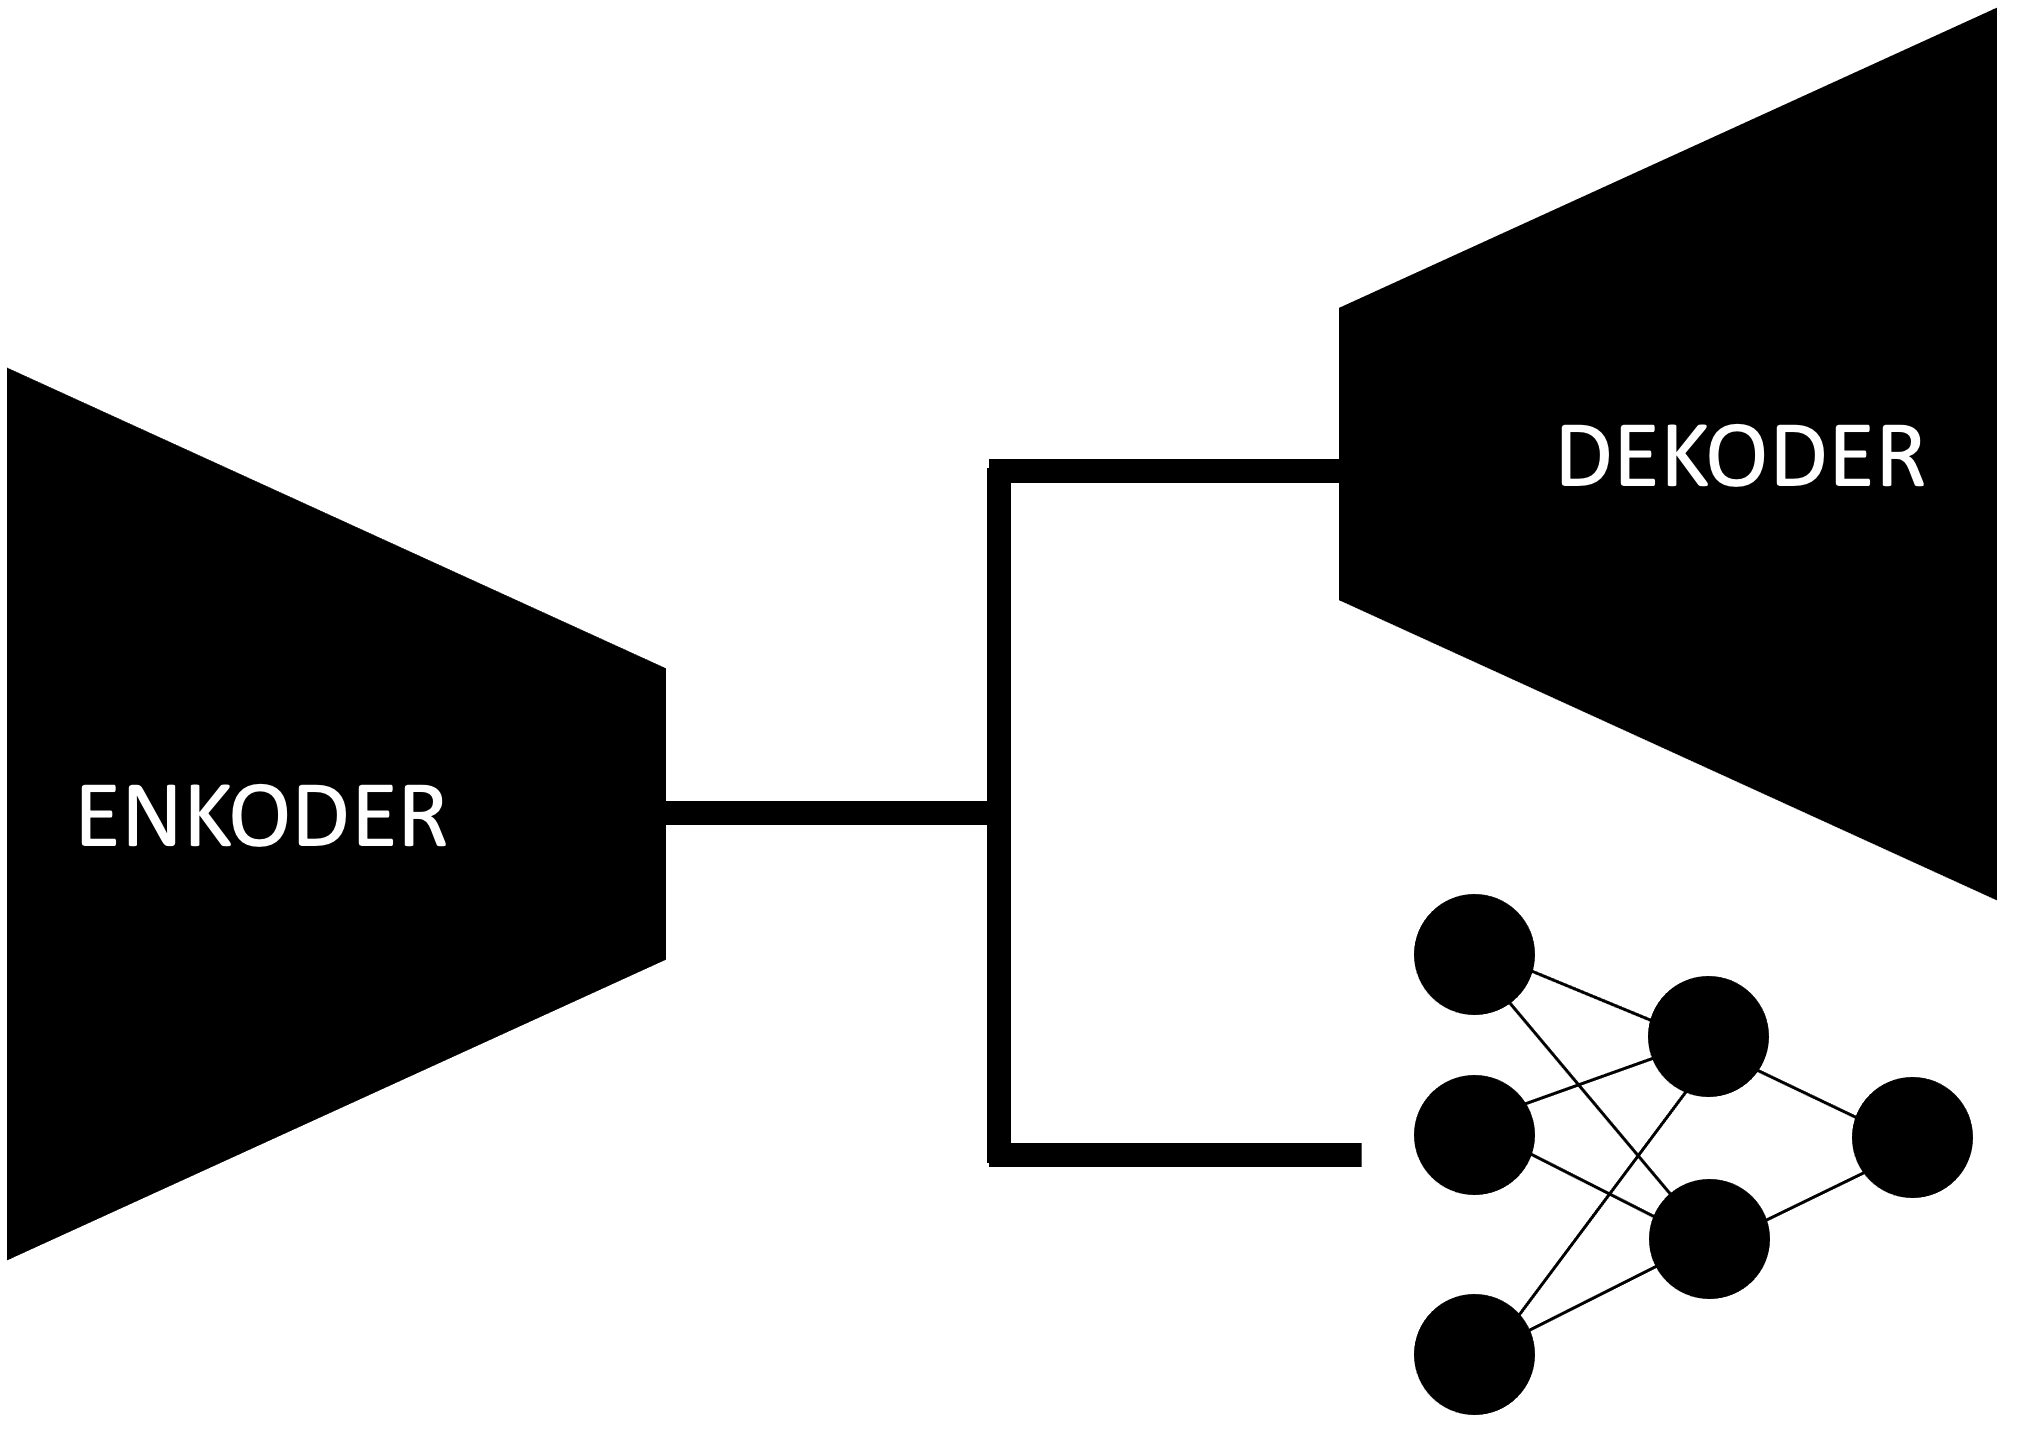
\includegraphics[width=\textwidth]{images/archs/multitask.png}
            \end{figure}
        \end{column}
    \end{columns}
\end{frame}

\begin{frame}{Opis eksperymentów}
    \begin{columns}
        \begin{column}{0.5\textwidth}
            \begin{itemize}
               \item Uczenie wielozadaniowe
               \item Finetuning
            \end{itemize}
        \end{column}

        \begin{column}{0.5\textwidth}
            \begin{figure}
                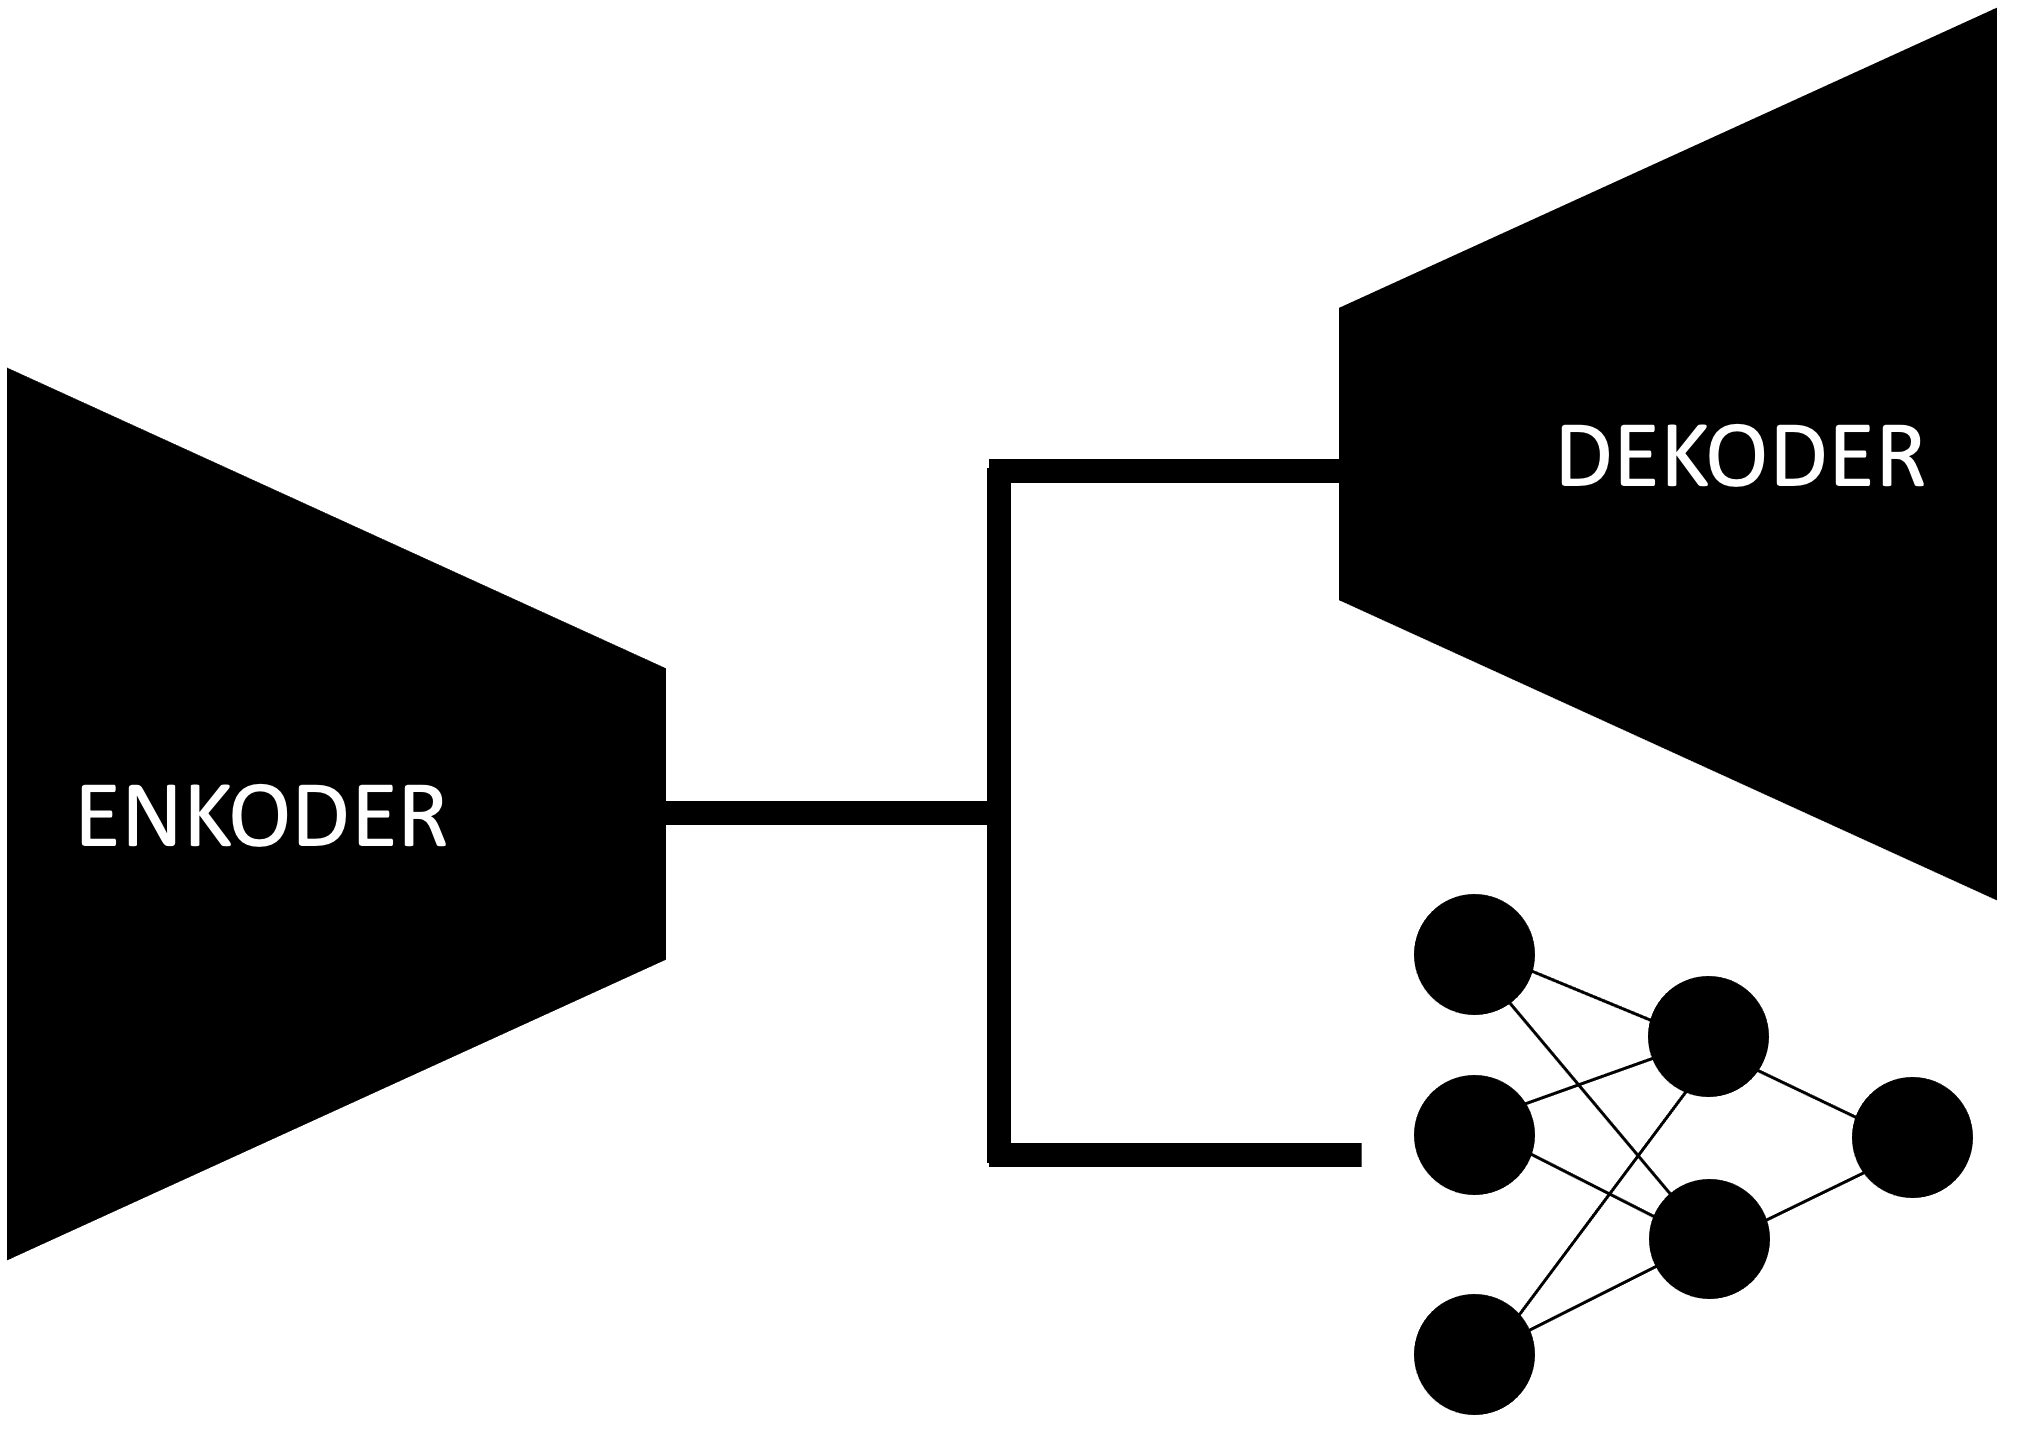
\includegraphics[width=\textwidth]{images/archs/multitask.png}
            \end{figure}
        \end{column}
    \end{columns}
\end{frame}\begin{frame}{Opis eksperymentów}
    \begin{columns}
        \begin{column}{0.5\textwidth}
            \begin{itemize}
               \item Uczenie wielozadaniowe
               \item Finetuning
               \item Wyłącznie klasyfikacja
            \end{itemize}
        \end{column}

        \begin{column}{0.5\textwidth}
            \begin{figure}
                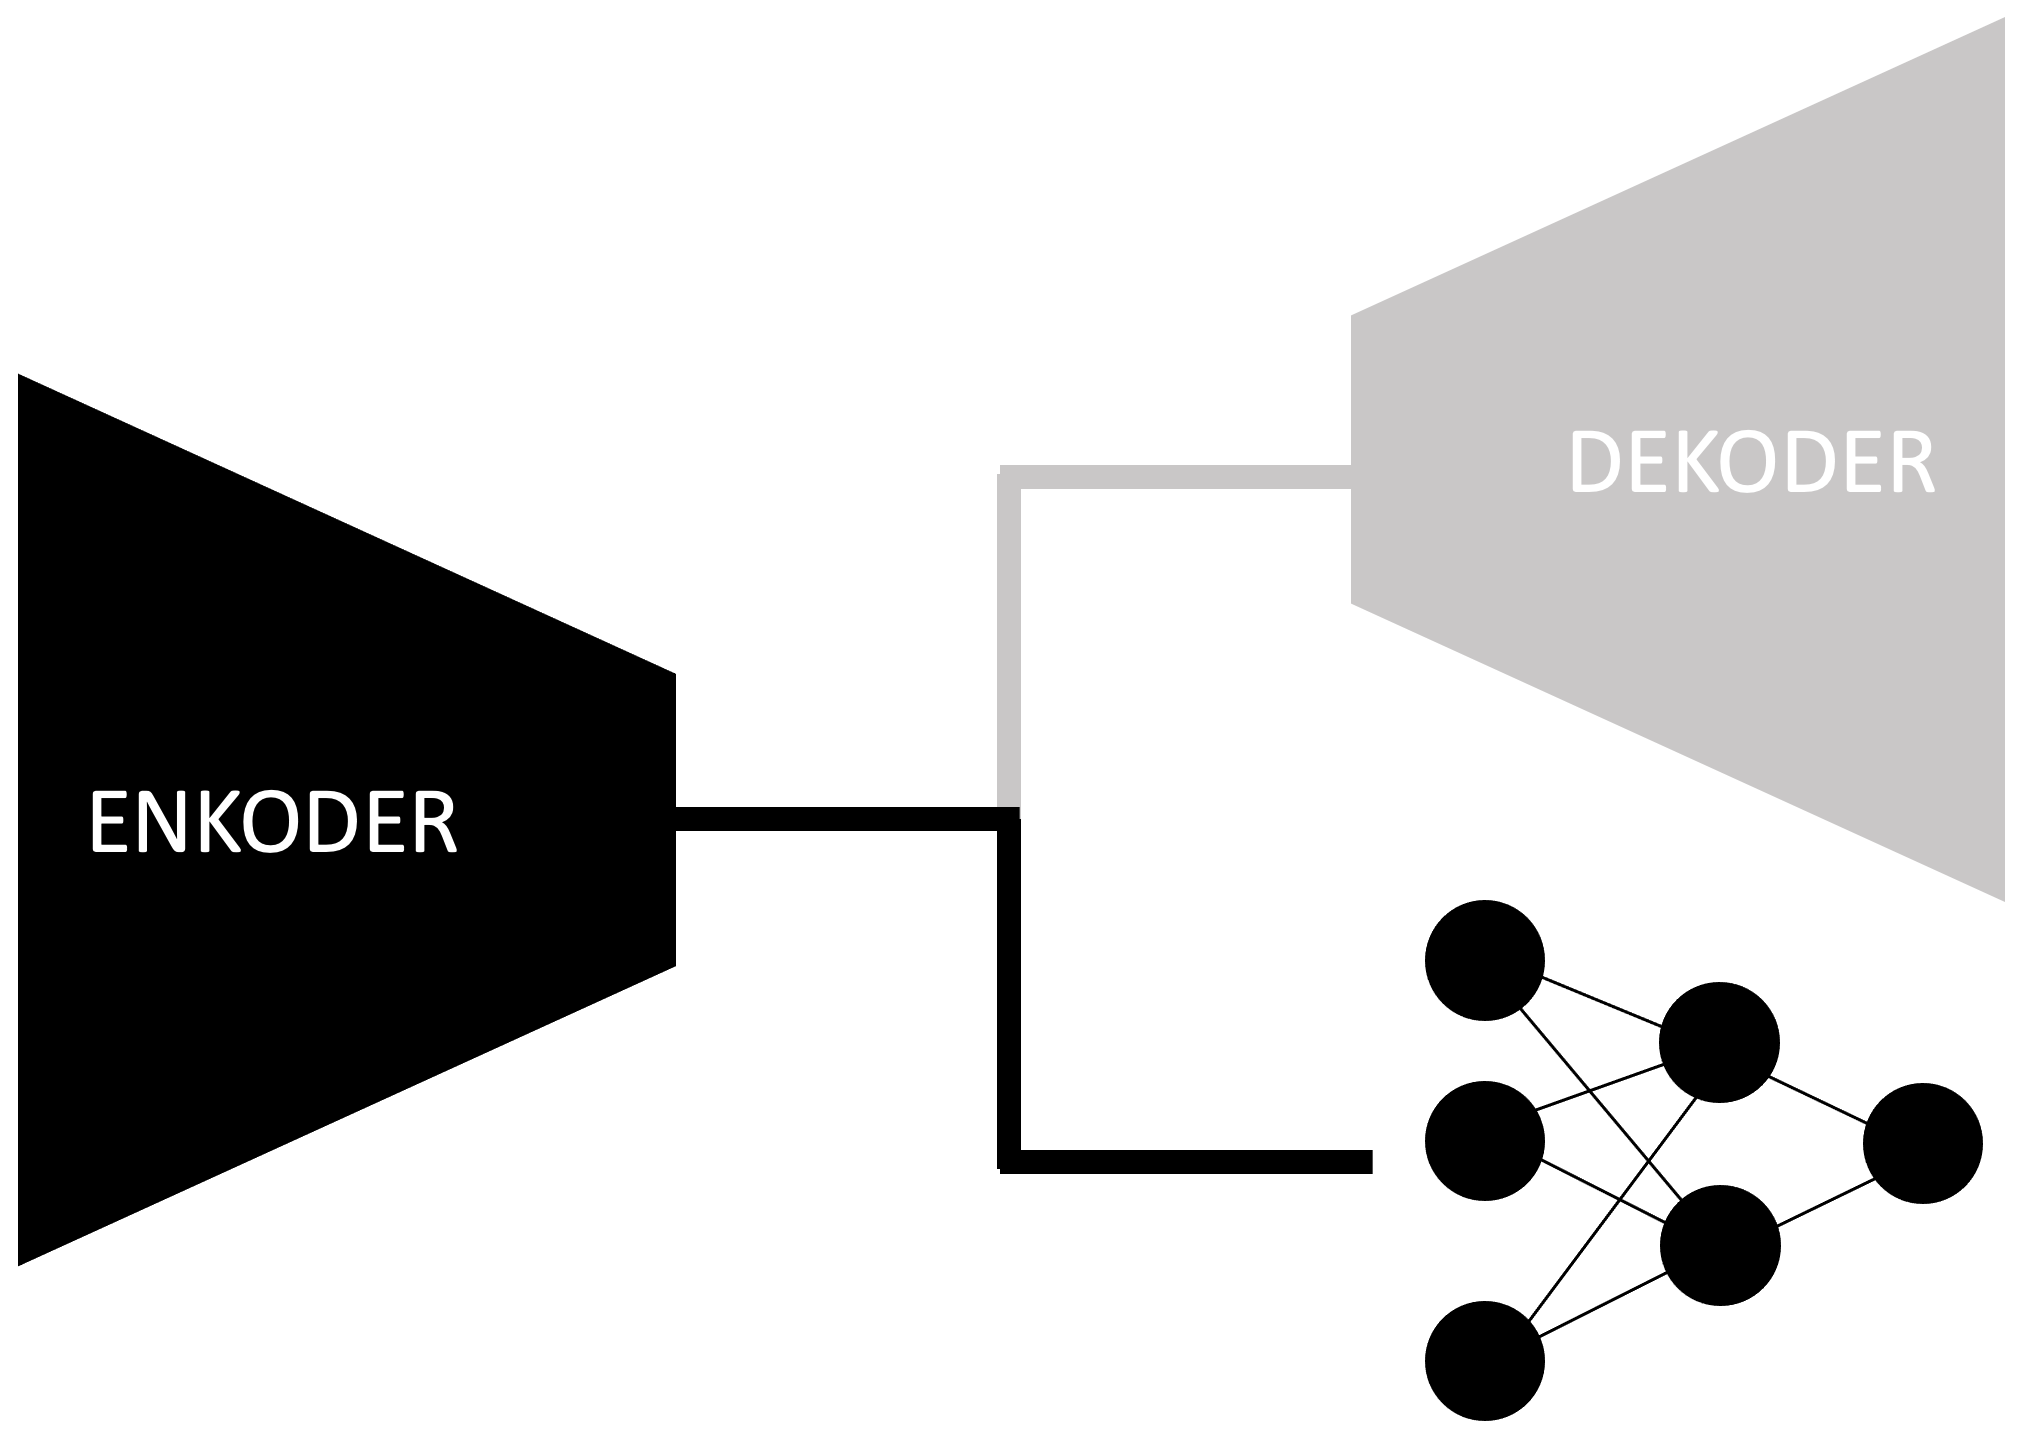
\includegraphics[width=\textwidth]{images/archs/only-classif.png}
            \end{figure}
        \end{column}
    \end{columns}
\end{frame}\begin{frame}{Opis eksperymentów}
    \begin{columns}
        \begin{column}{0.5\textwidth}
            \begin{itemize}
               \item Uczenie wielozadaniowe
               \item Finetuning
               \item Wyłącznie klasyfikacja
               \item Wyłącznie segmentacja
            \end{itemize}
        \end{column}

        \begin{column}{0.5\textwidth}
            \begin{figure}
                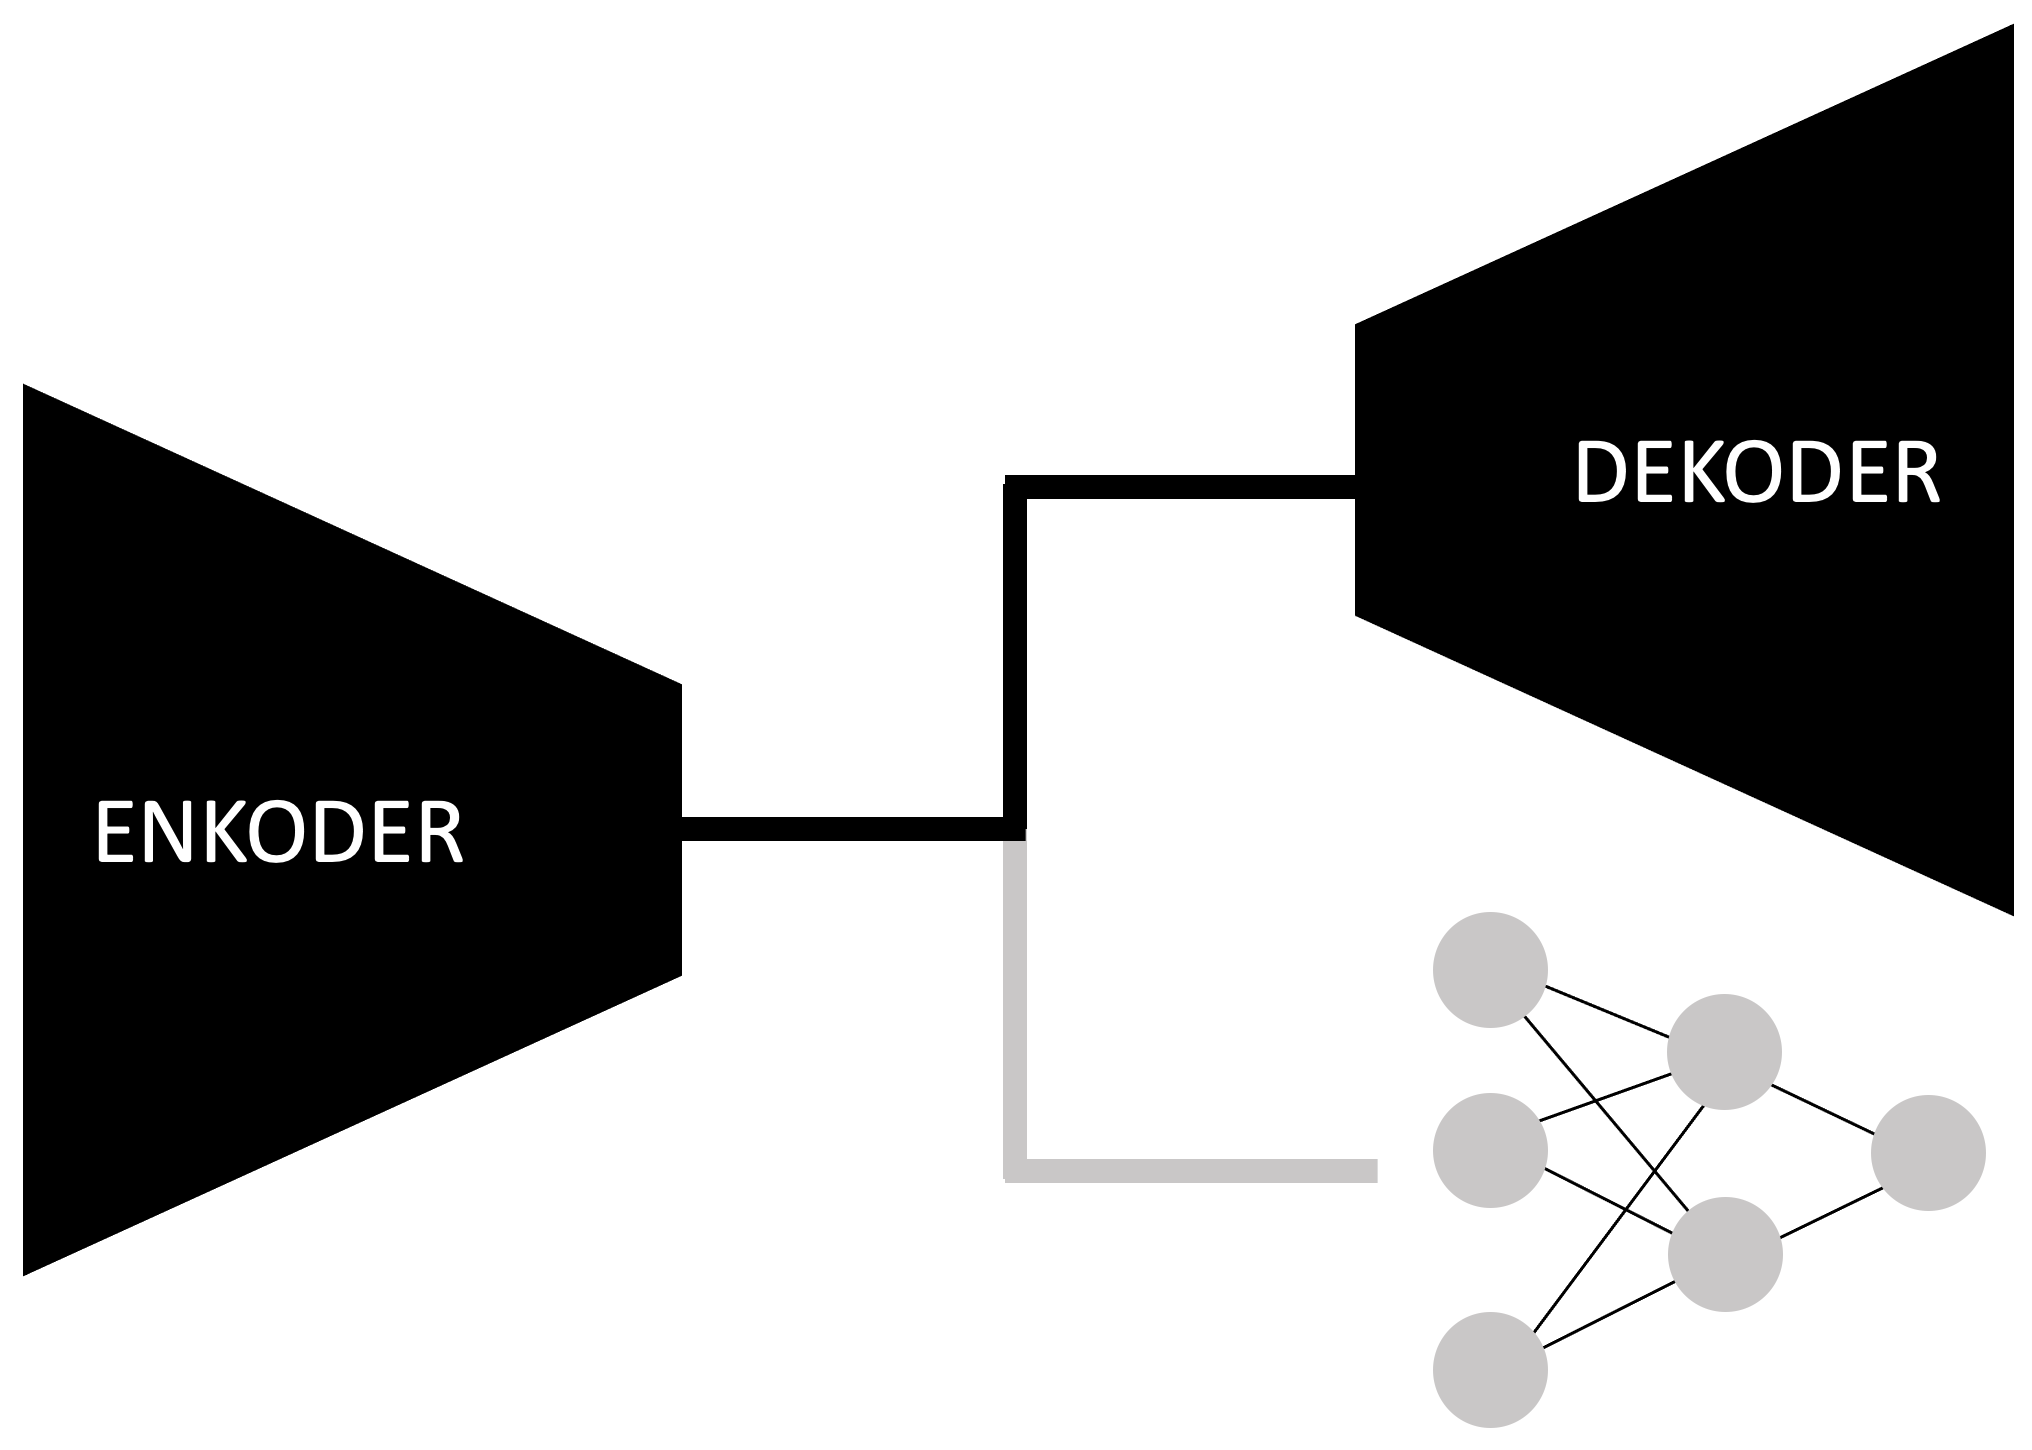
\includegraphics[width=\textwidth]{images/archs/only-segm.png}
            \end{figure}
        \end{column}
    \end{columns}
\end{frame}\begin{frame}{Opis eksperymentów}
    \begin{columns}
        \begin{column}{0.5\textwidth}
            \begin{itemize}
               \item Uczenie wielozadaniowe
               \item Finetuning
               \item Wyłącznie klasyfikacja
               \item Wyłącznie segmentacja
               \item Pośrednia klasyfikacja z~segmentacji
            \end{itemize}
        \end{column}

        \begin{column}{0.5\textwidth}
            \begin{figure}
                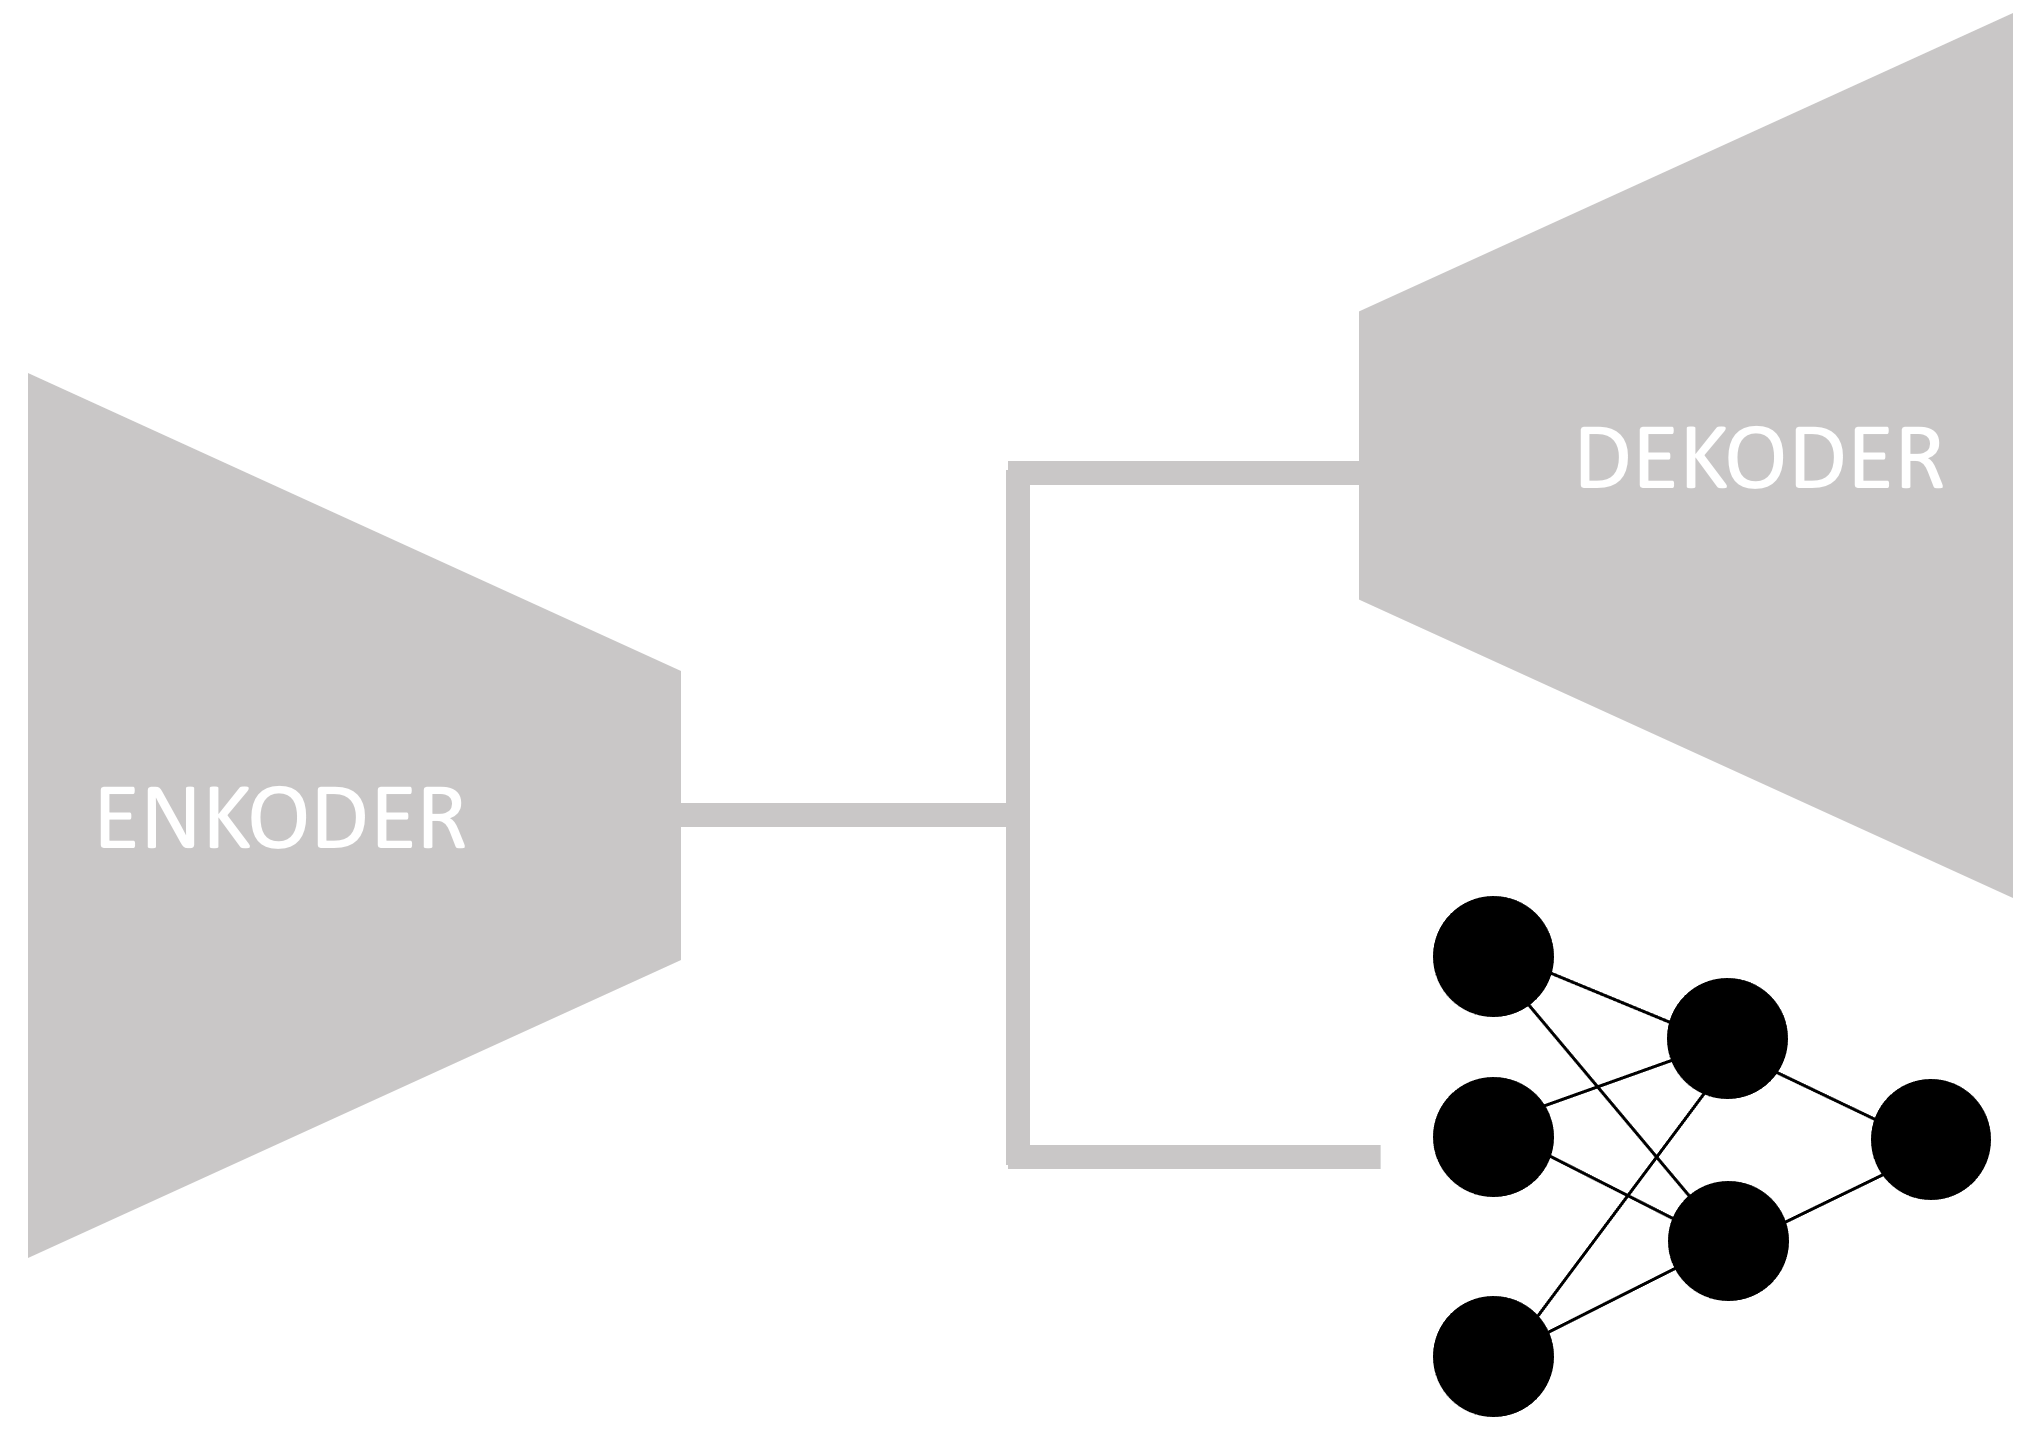
\includegraphics[width=\textwidth]{images/archs/indirect-classif.png}
            \end{figure}
        \end{column}
    \end{columns}
\end{frame}\begin{frame}{Opis eksperymentów}
    \begin{columns}
        \begin{column}{0.5\textwidth}
            \begin{itemize}
               \item Uczenie wielozadaniowe
               \item Finetuning
               \item Wyłącznie klasyfikacja
               \item Wyłącznie segmentacja
               \item Pośrednia klasyfikacja z~segmentacji
               \item Bezpośrednia klasyfikacja z~segmentacji
            \end{itemize}
        \end{column}

        \begin{column}{0.5\textwidth}
            \begin{figure}
                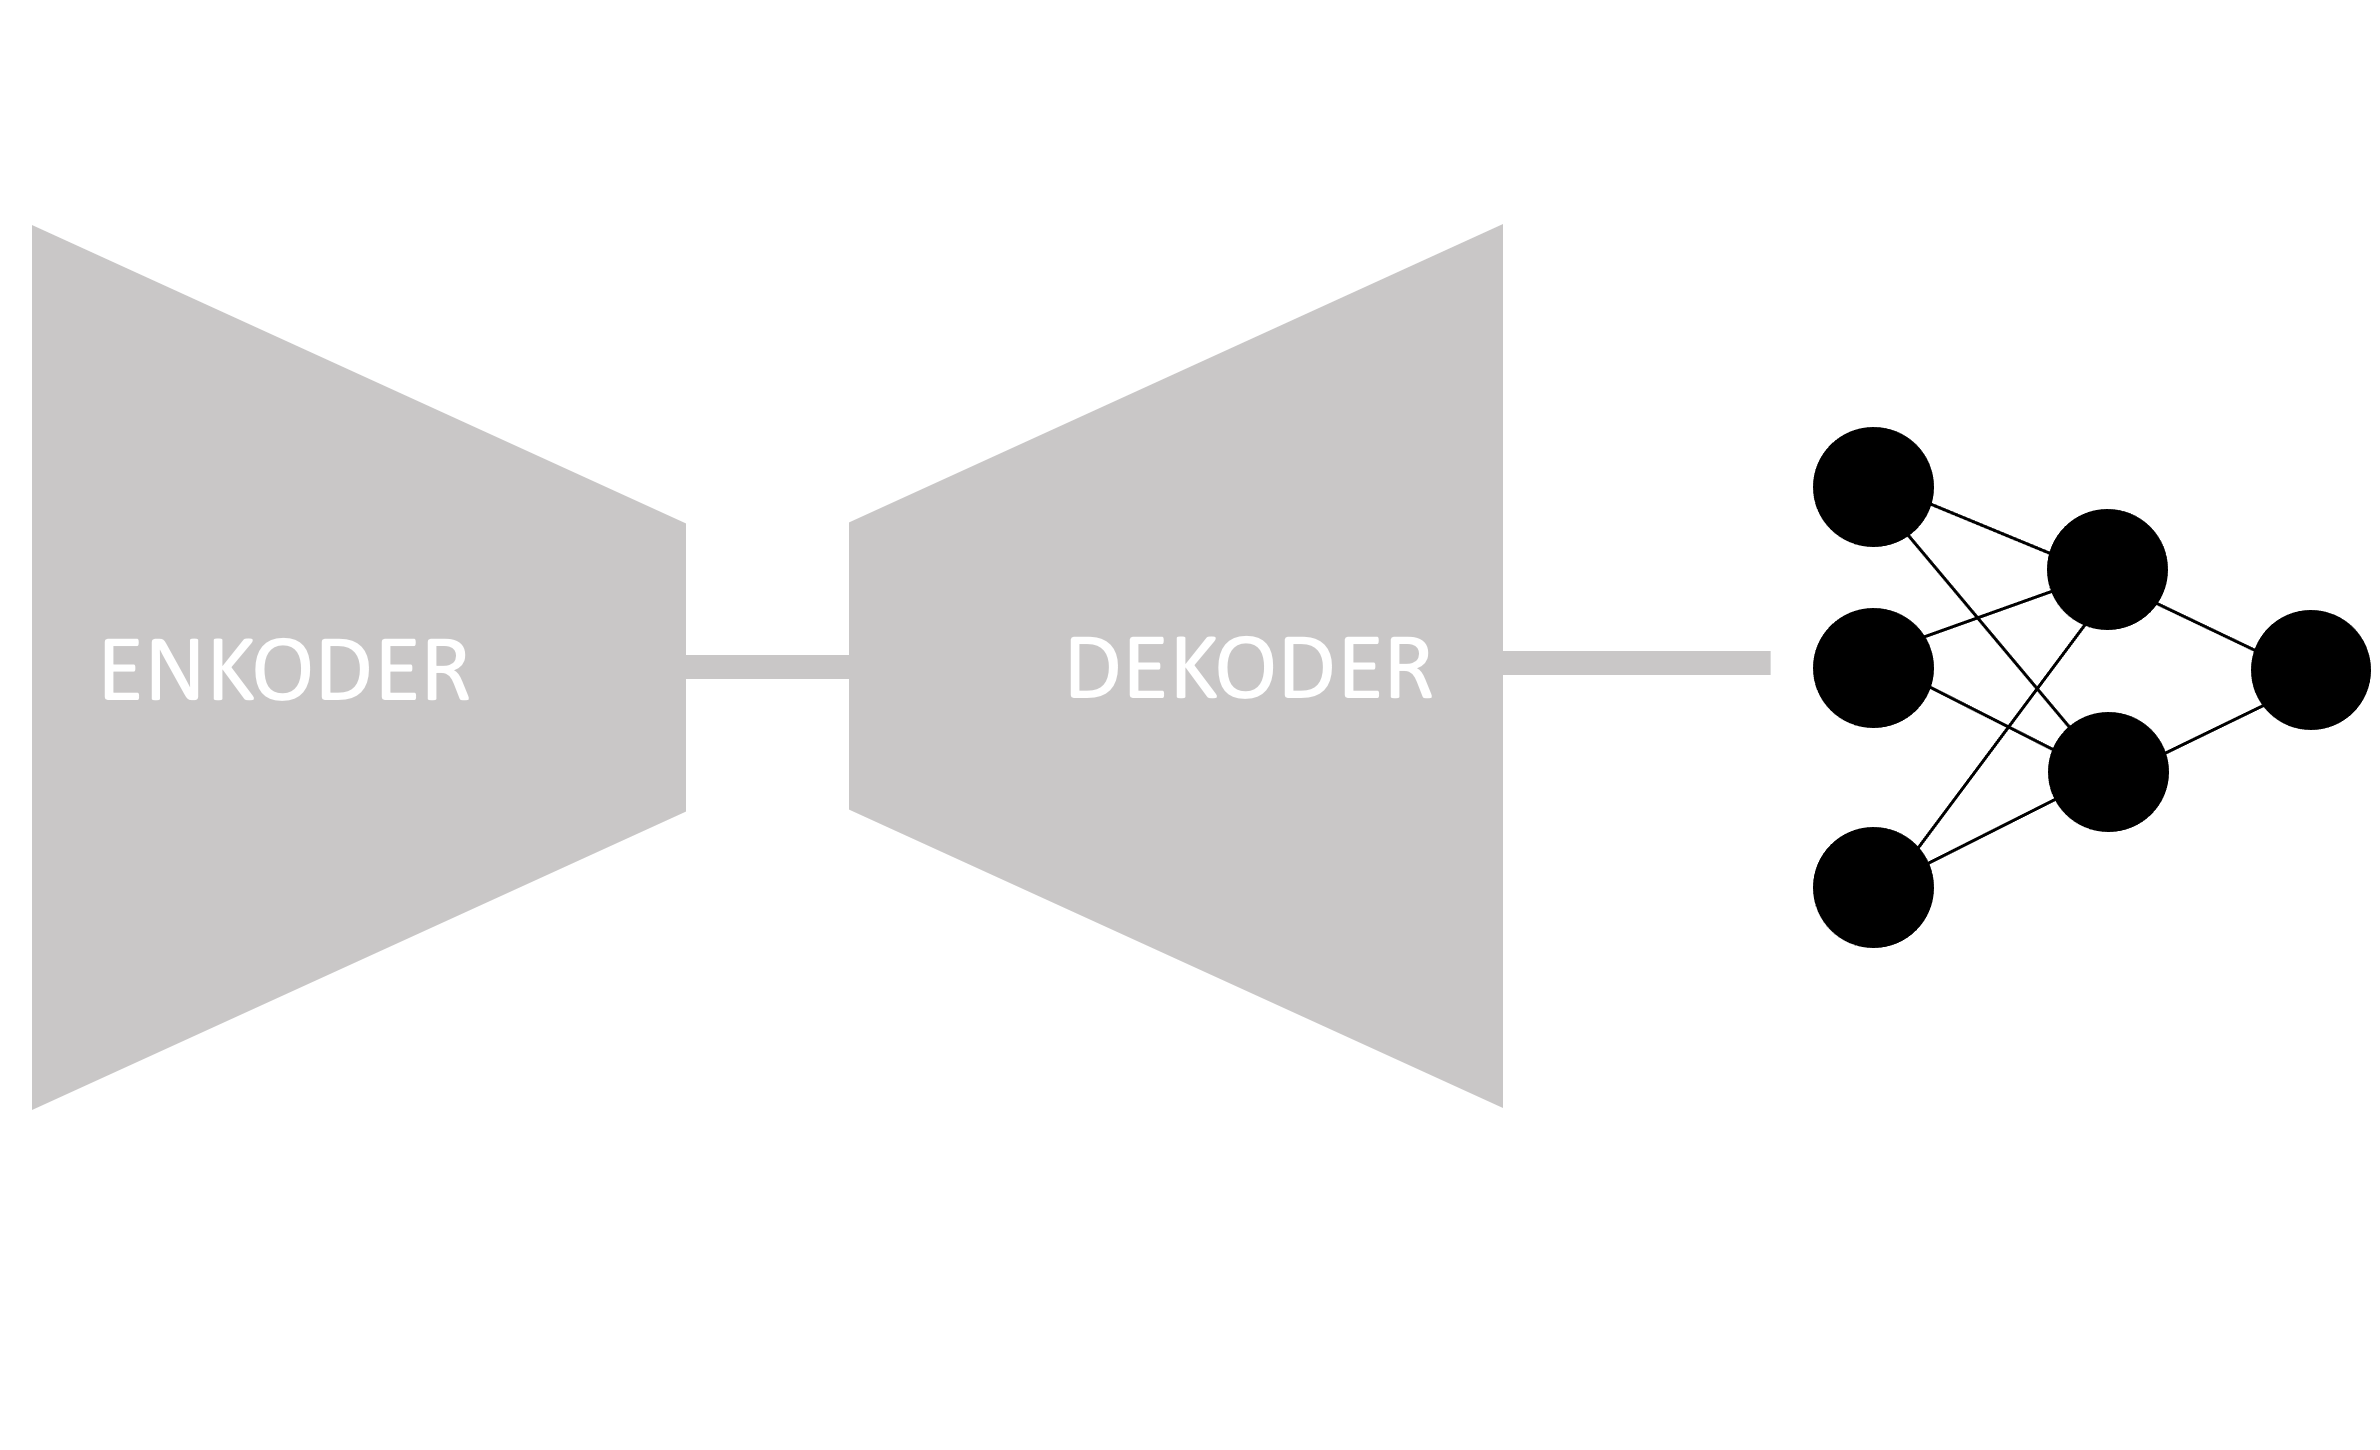
\includegraphics[width=\textwidth]{images/archs/direct-classif.png}
            \end{figure}
        \end{column}
    \end{columns}
\end{frame}

\section*{Wyniki}
\section*{Analiza jakościowa}
\begin{frame}{Klasyfikacja sceny}
    
    \begin{figure}[ht!]
        \centering
        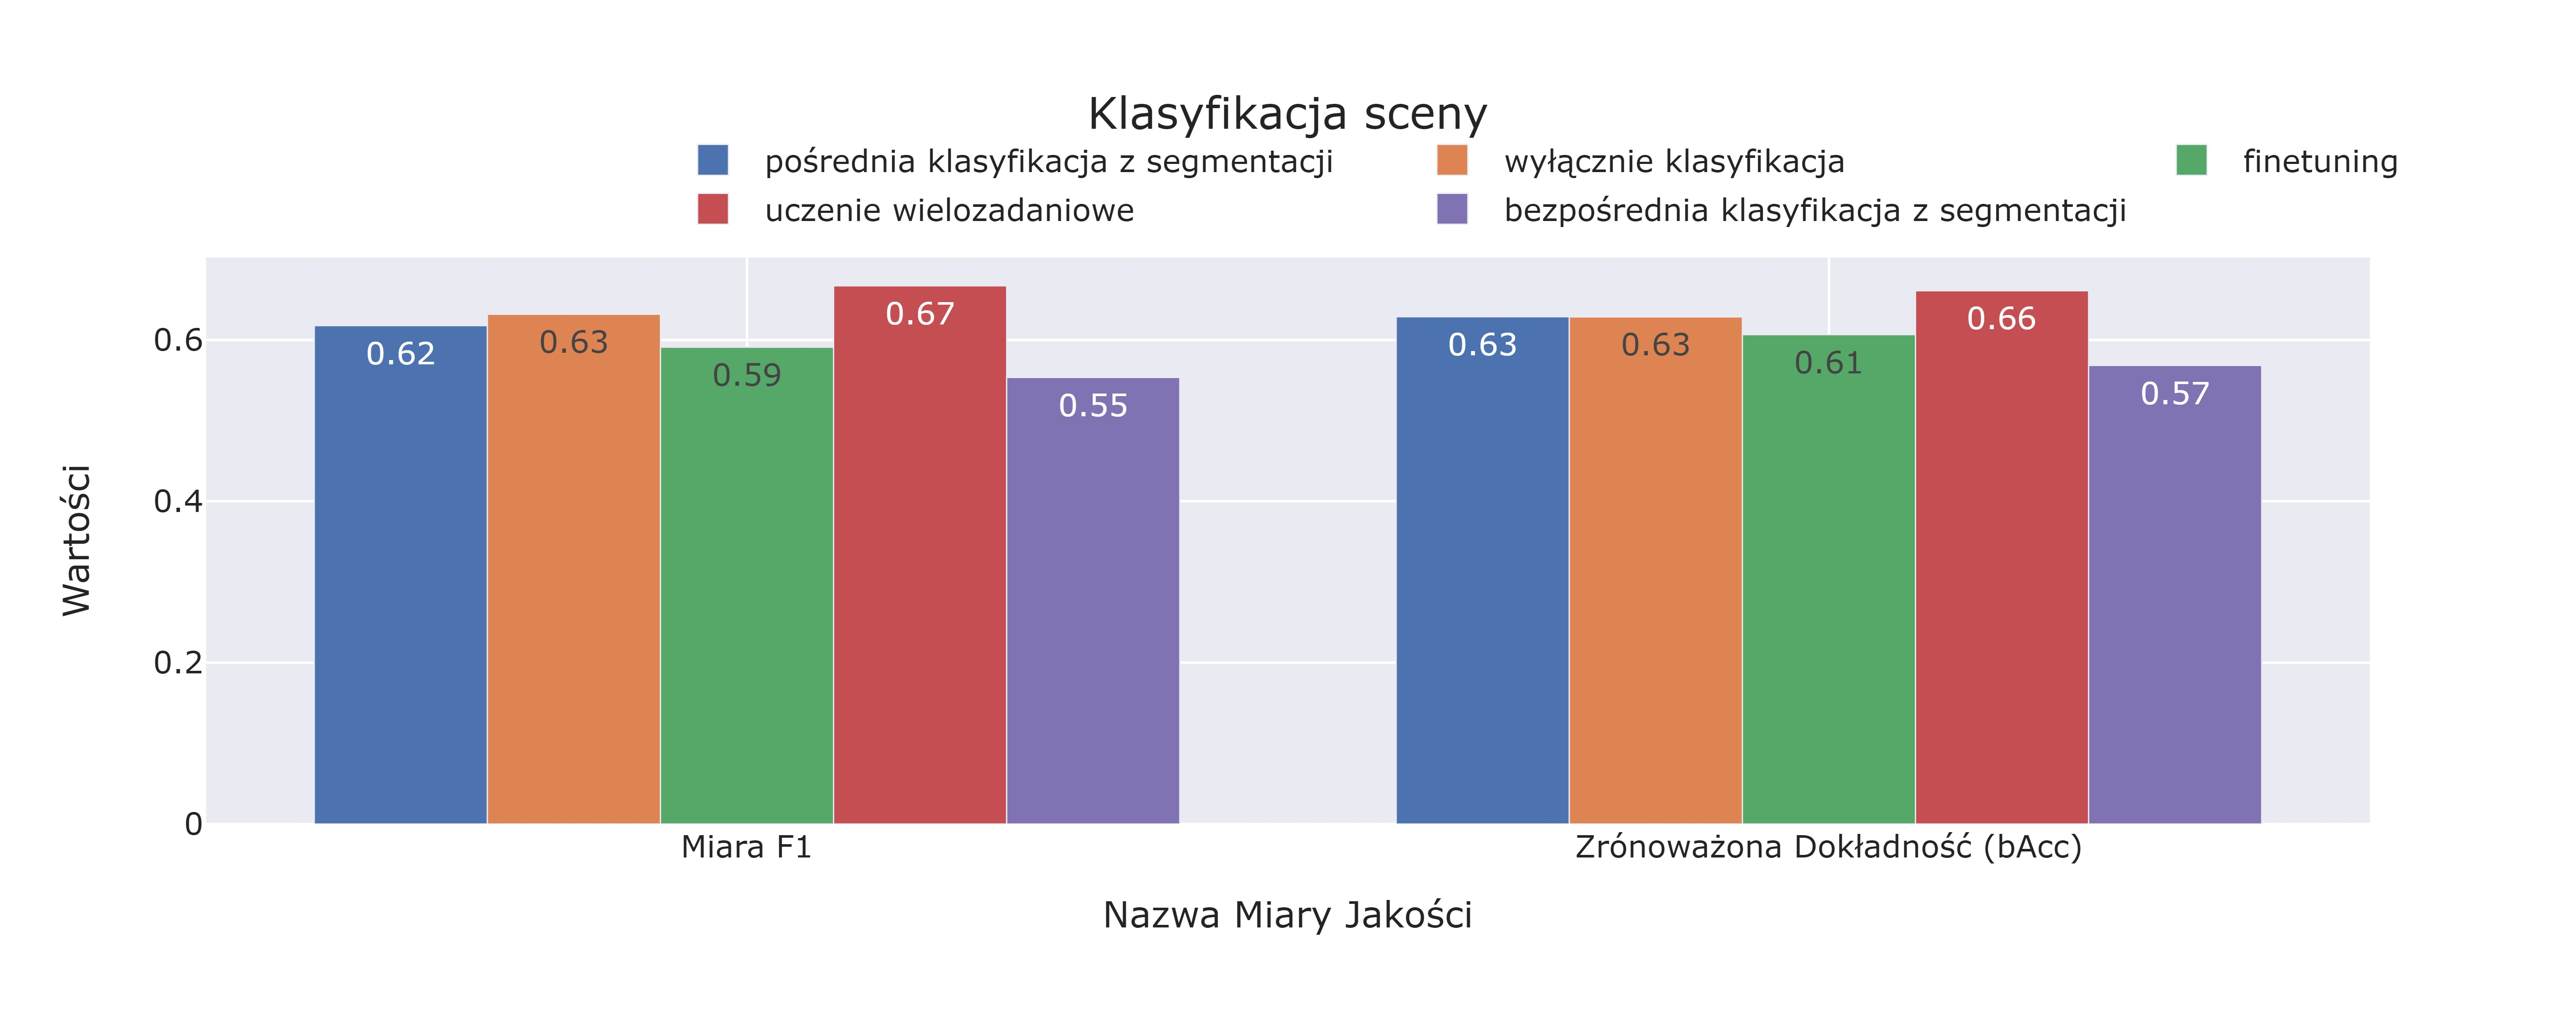
\includegraphics[width=\textwidth]{images/pl-res/Klasyfikacja-sceny.jpeg}
        \caption{Porównanie miar F1 oraz dokładnosci dla klasyfikacji sceny.}
        \label{fig:macro-classification}
    \end{figure}
\end{frame}

\begin{frame}{Segmentacja semantyczna}
    
    \begin{figure}[ht!]
        \centering
        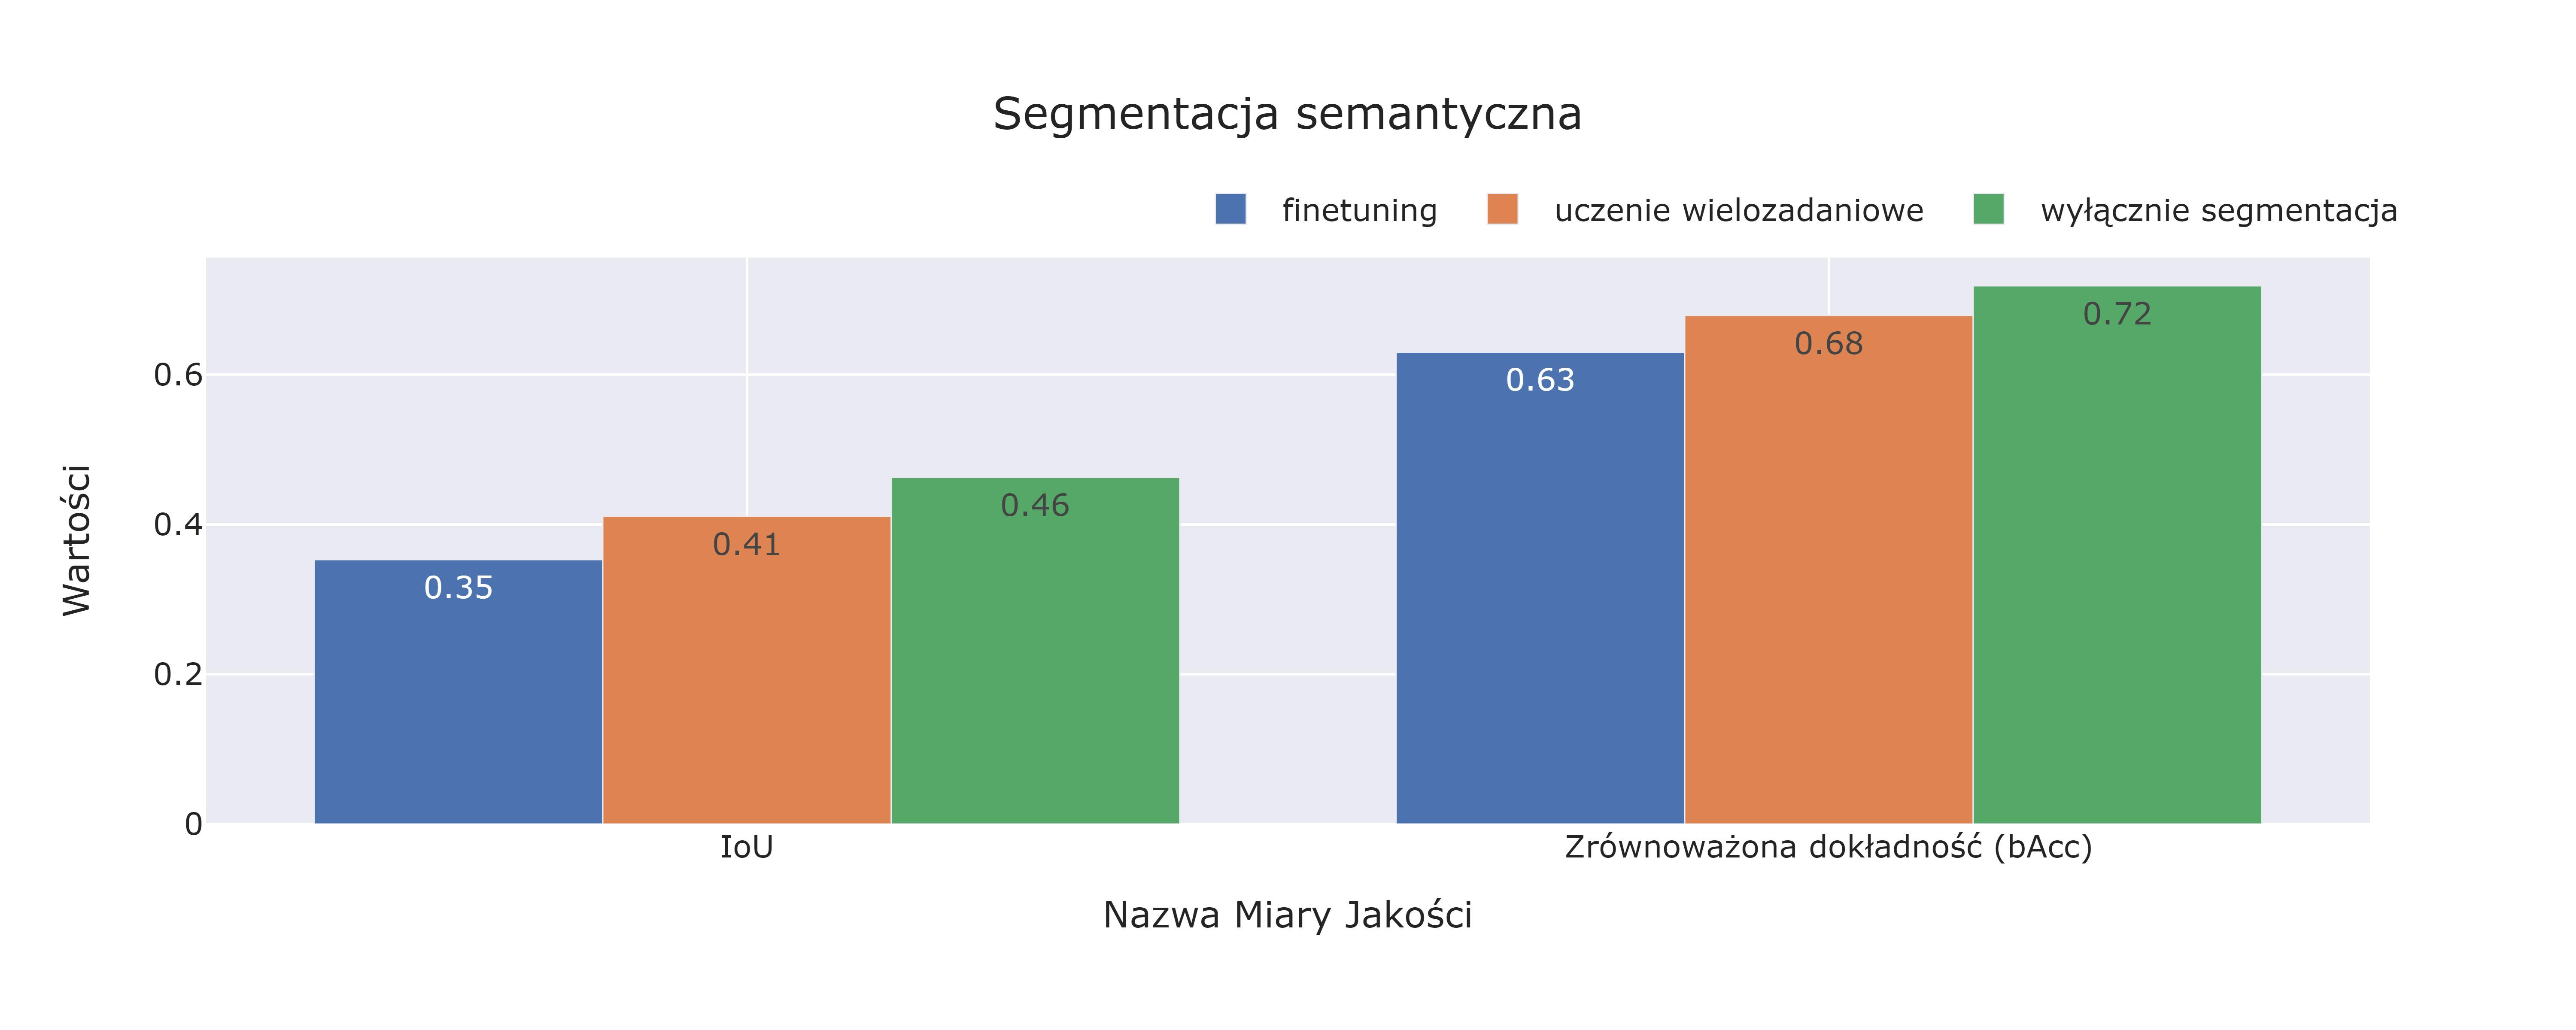
\includegraphics[width=\textwidth]{images/pl-res/Segmentacja-semantyczna.jpeg}
        \caption{Porównanie miar IoU oraz dokładnosci dla segmentacji sceny.}
        \label{fig:macro-segmentation}
    \end{figure}
\end{frame}
\section*{Analiza wydajnościowa}
\begin{frame}{Analiza czasu uczenia}
    \begin{table}[ht!]
        \centering
        \begin{tabular}{c|c}
            nazwa zadania                      &   $\approx$ czas{[}s{]} \\ \hline
            wyłącznie segmentacja +  wyłącznie klasyfikacja &  360 \\
            wyłącznie segmetnacja + pośrednia klasyfikacja &  260 \\
            wyłącznie segmetnacja + bezpośrednia klasyfikacja &  275 \\
            uczenie wielozadaniowe                   &    211 \\
            finetuning                        &    160 
    \end{tabular}
    \caption{Porównanie czasu uczenia względem całości.}
    \label{tab:por-trening-all}
    \end{table}
\end{frame}

\begin{frame}{Analiza czasu wnioskowania}
    
    \begin{table}[ht!]
        \centering
        \begin{tabular}{c|c}
            rodzaj sieci                      &   czas{[}s{]} \\ \hline
            dwie szeregowe sieci                  &   15.7\\
            jedna architektura               &   8.6
    \end{tabular}
    \caption{Porównanie czasu wnioskowania.}
    \label{tab:por-infer}
    \end{table}
\end{frame}

\begin{frame}{Wyniki}
    \begin{block}{Wady}
        \begin{itemize}
            \item Pogorszenie segmentacji
        \end{itemize}
    \end{block}


    \begin{block}{Zalety}
        \begin{itemize}
            \item Poprawa klasyfikacji
            \item Skrócenie czasu uczenia
            \item Dwukrotne skórcenie czasu wnioskowania
        \end{itemize}
    \end{block}
    
\end{frame}

\begin{frame}{Podsumowanie}
    Cel pracy został spełniony, dodatkowo odpowiadając na inne pytania badawcze.
    \begin{itemize}
        \item Jak można zaprojektować model oparty na głębokim uczeniu do wspólnej segmentacji semantycznej i klasyfikacji scen w środowiskach wewnętrznych?
        \item Czy przestrzeń reprezentacji po wytrenowaniu na zadaniu segmentacji semantycznej może być użyta do zadania klasyfikacji sceny?
        \item Jak dobrze proponowany model radzi sobie na dużym zbiorze danych scen wewnętrznych i jak wypada w porównaniu z aktualnymi metodami segmentacji semantycznej i klasyfikacji scen osobno?
        \item Jak proponowany model może być wykorzystany do poprawy wydajności w robotyce mobilnej?
    \end{itemize}

    

\end{frame}
\begin{frame}[plain, allowframebreaks,noframenumbering]{Bibliografia}
    
    \bibliography{presentation}
    \bibliographystyle{abbrv}
    
\end{frame}


\appendix

\begin{frame}{Obraz}
    \begin{figure}[ht!]
        \centering
        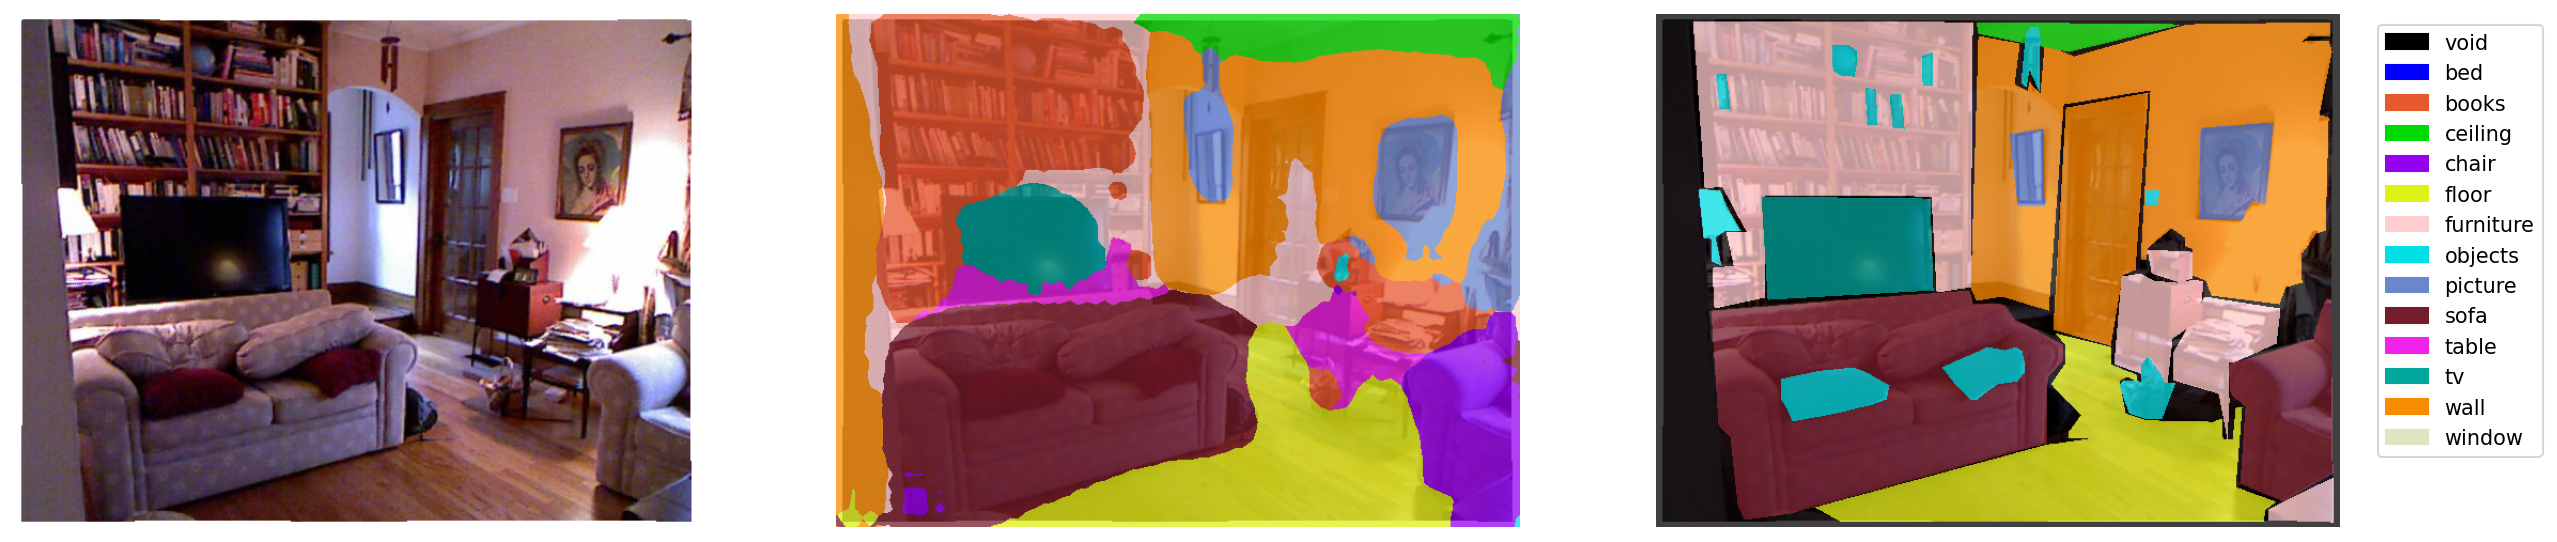
\includegraphics[width=\textwidth]{images/living_room-1.png}
        \caption{Porównanie jakości segmentacji dla klasy salon.}
        \label{fig:living_room-pred-1}
    \end{figure}
\end{frame}
\begin{frame}{Architektura wielozadaniowa}
    \begin{figure}[ht!]
    \centering
    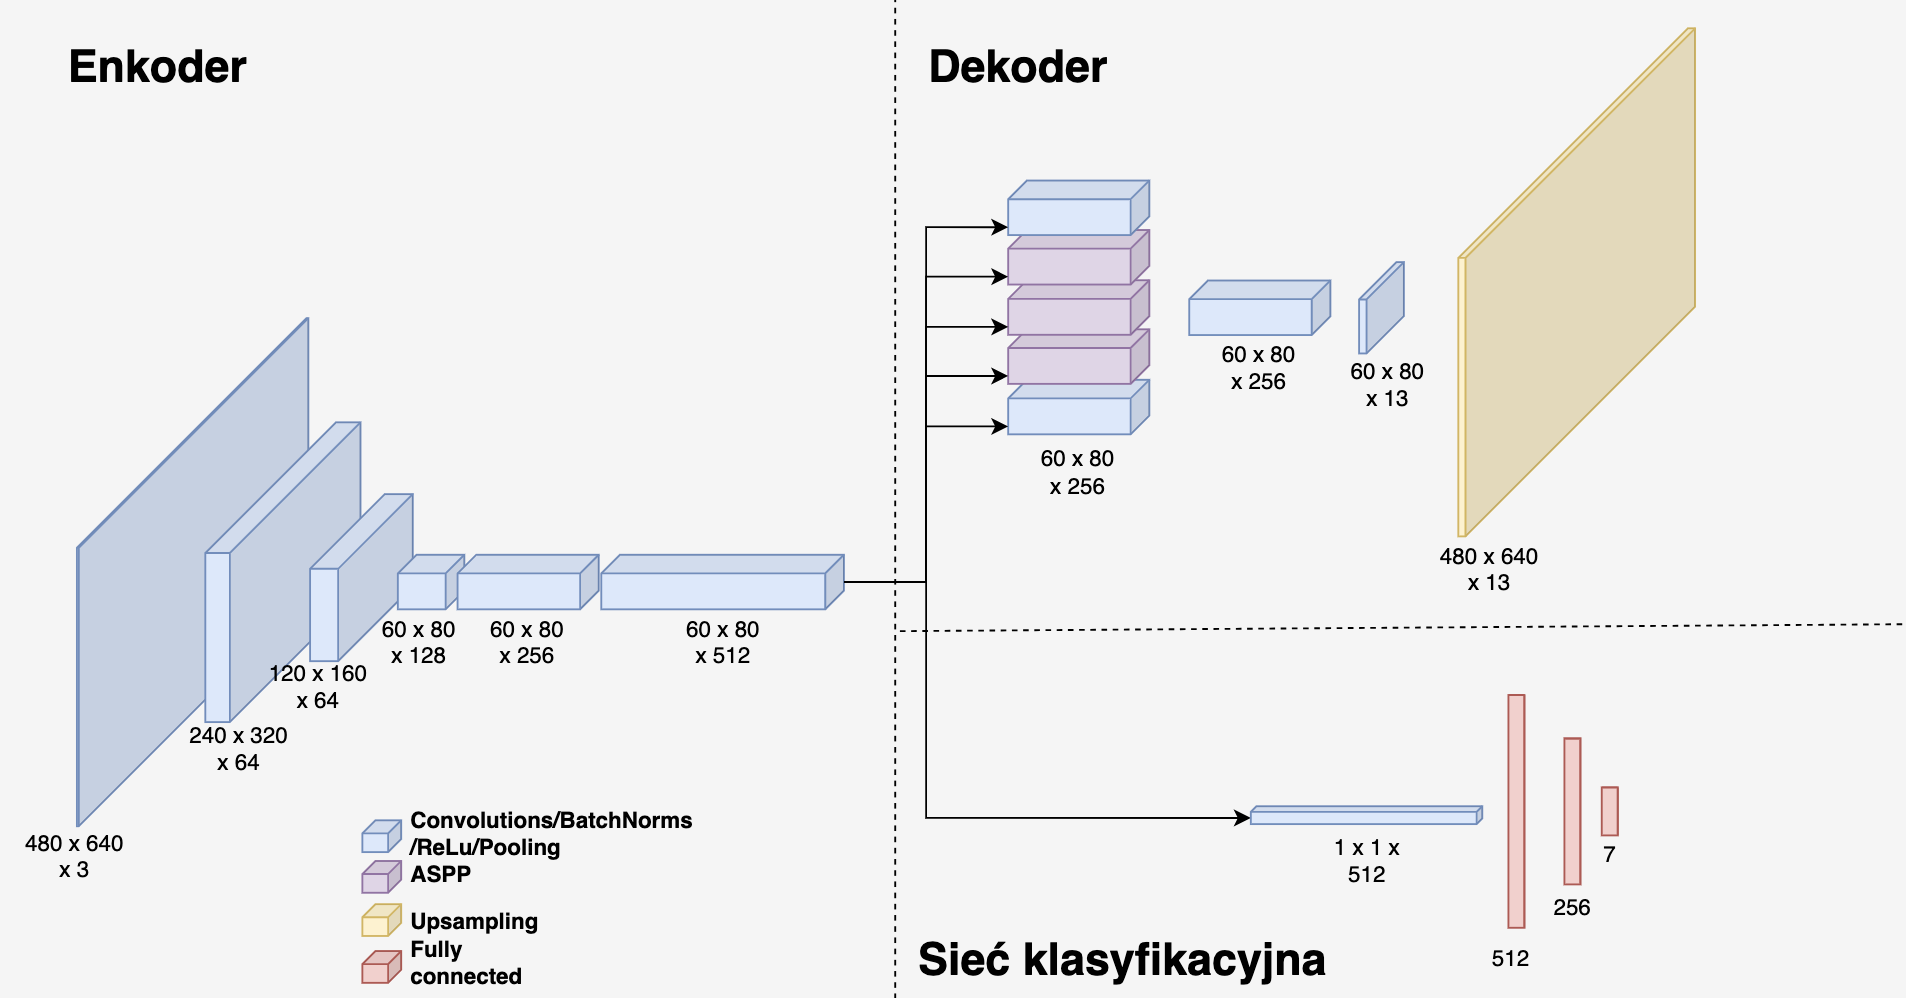
\includegraphics[width=\textwidth]{images/multitask-arch-new.png}
    \caption{Architektura wielozadaniowej sieci.}
    \label{fig:multitask}
    \end{figure}
    
\end{frame}
\begin{frame}{Miary jakości klasyfikacji}
    
    \begin{figure}[ht!]
        \centering
        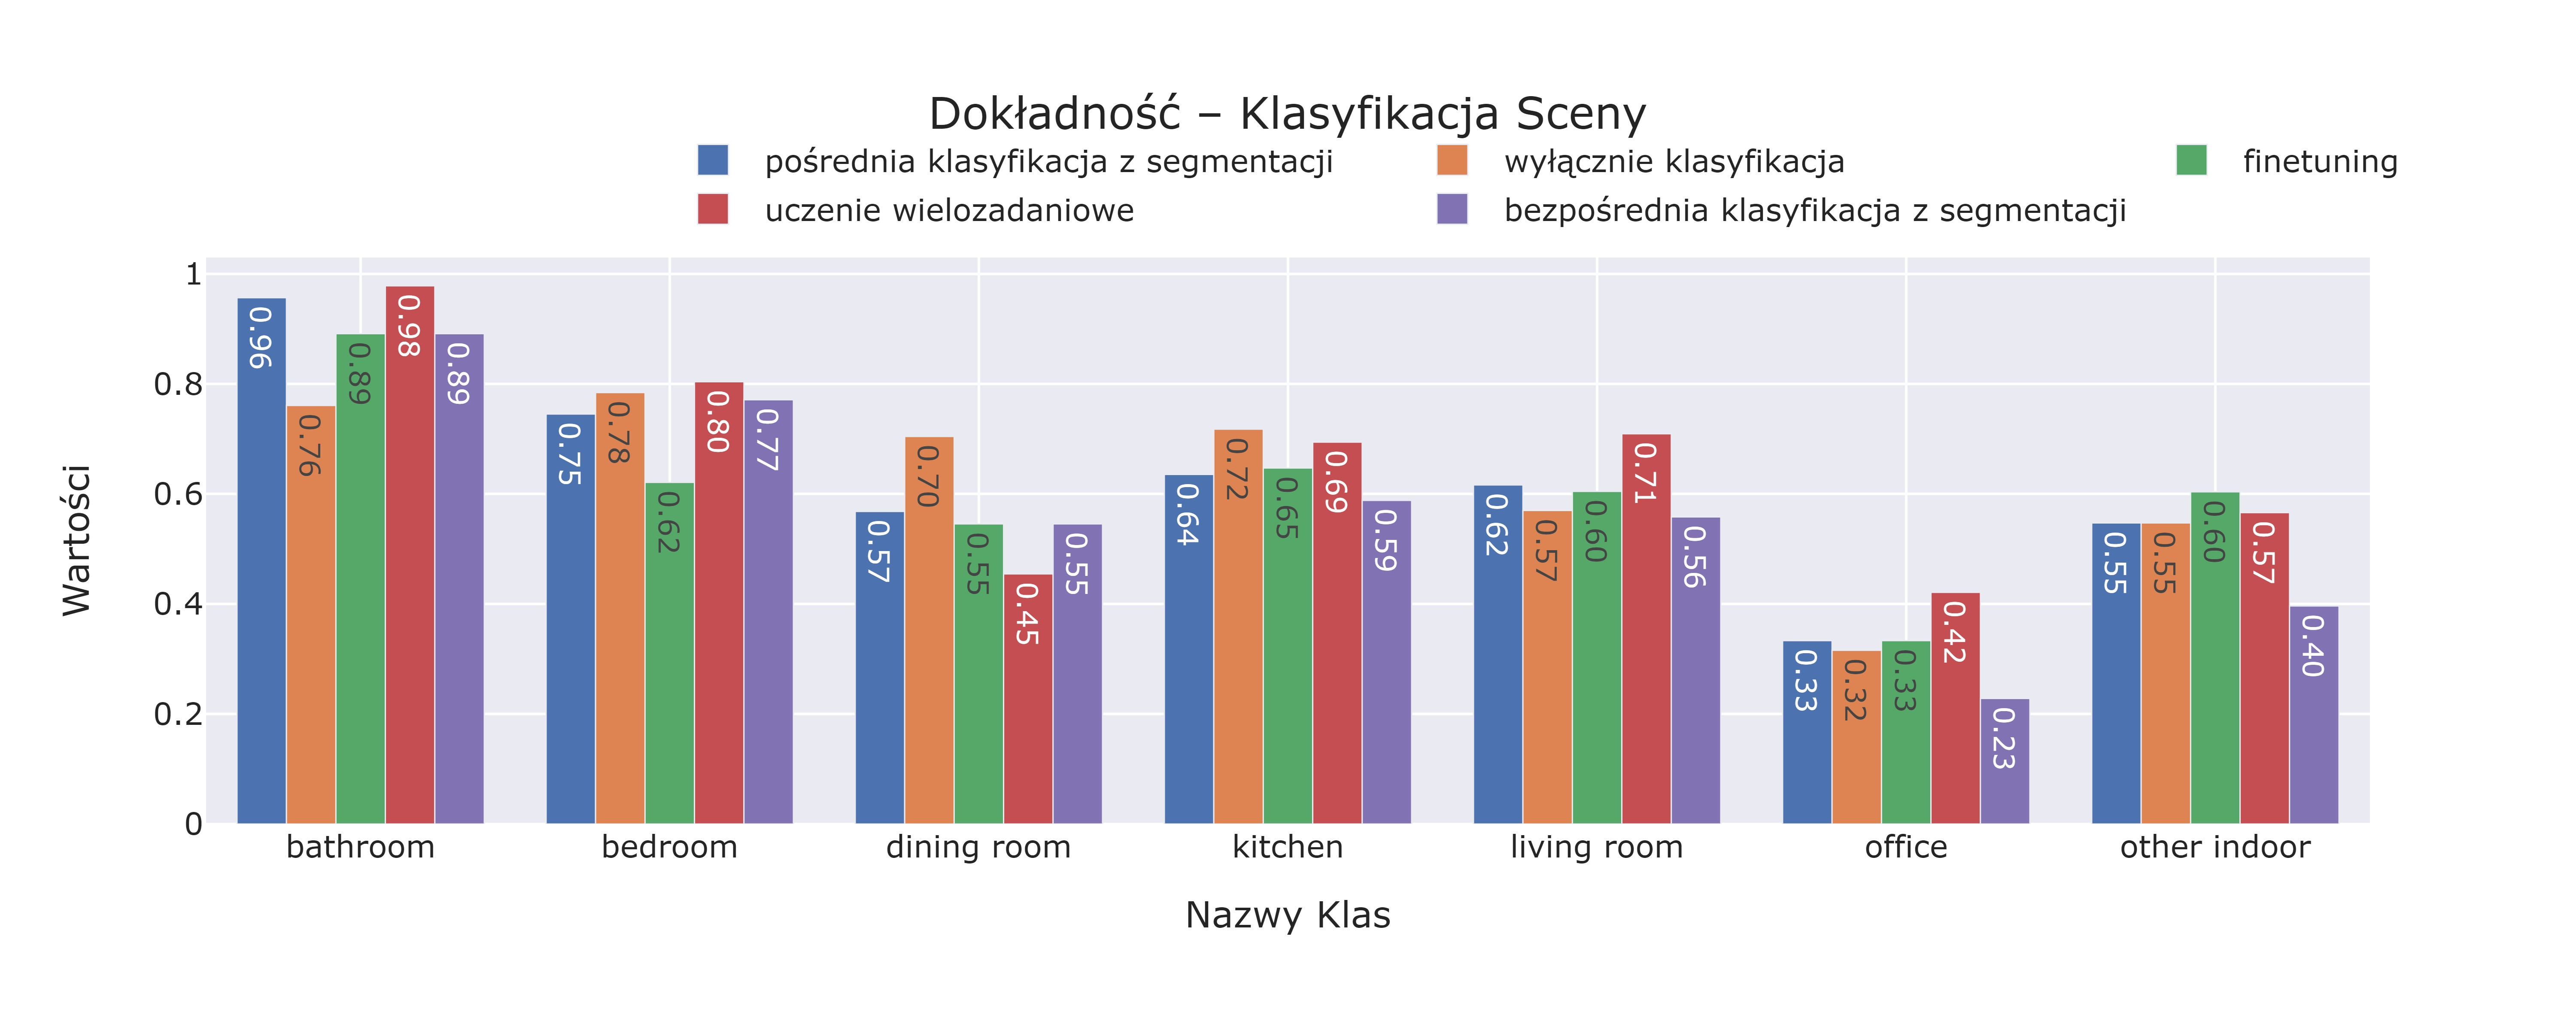
\includegraphics[width=\textwidth]{images/pl-res/Dokladnosc-Klasyfikacja-Sceny.jpeg}
        \caption{Porównanie dokładności klasyfikacji sceny z rozróżniem konkretnych klas.}
        \label{fig:classification-accuracy}
    \end{figure}
\end{frame}


\begin{frame}{Miary jakości klasyfikacji}
    
    \begin{figure}[ht!]
        \centering
        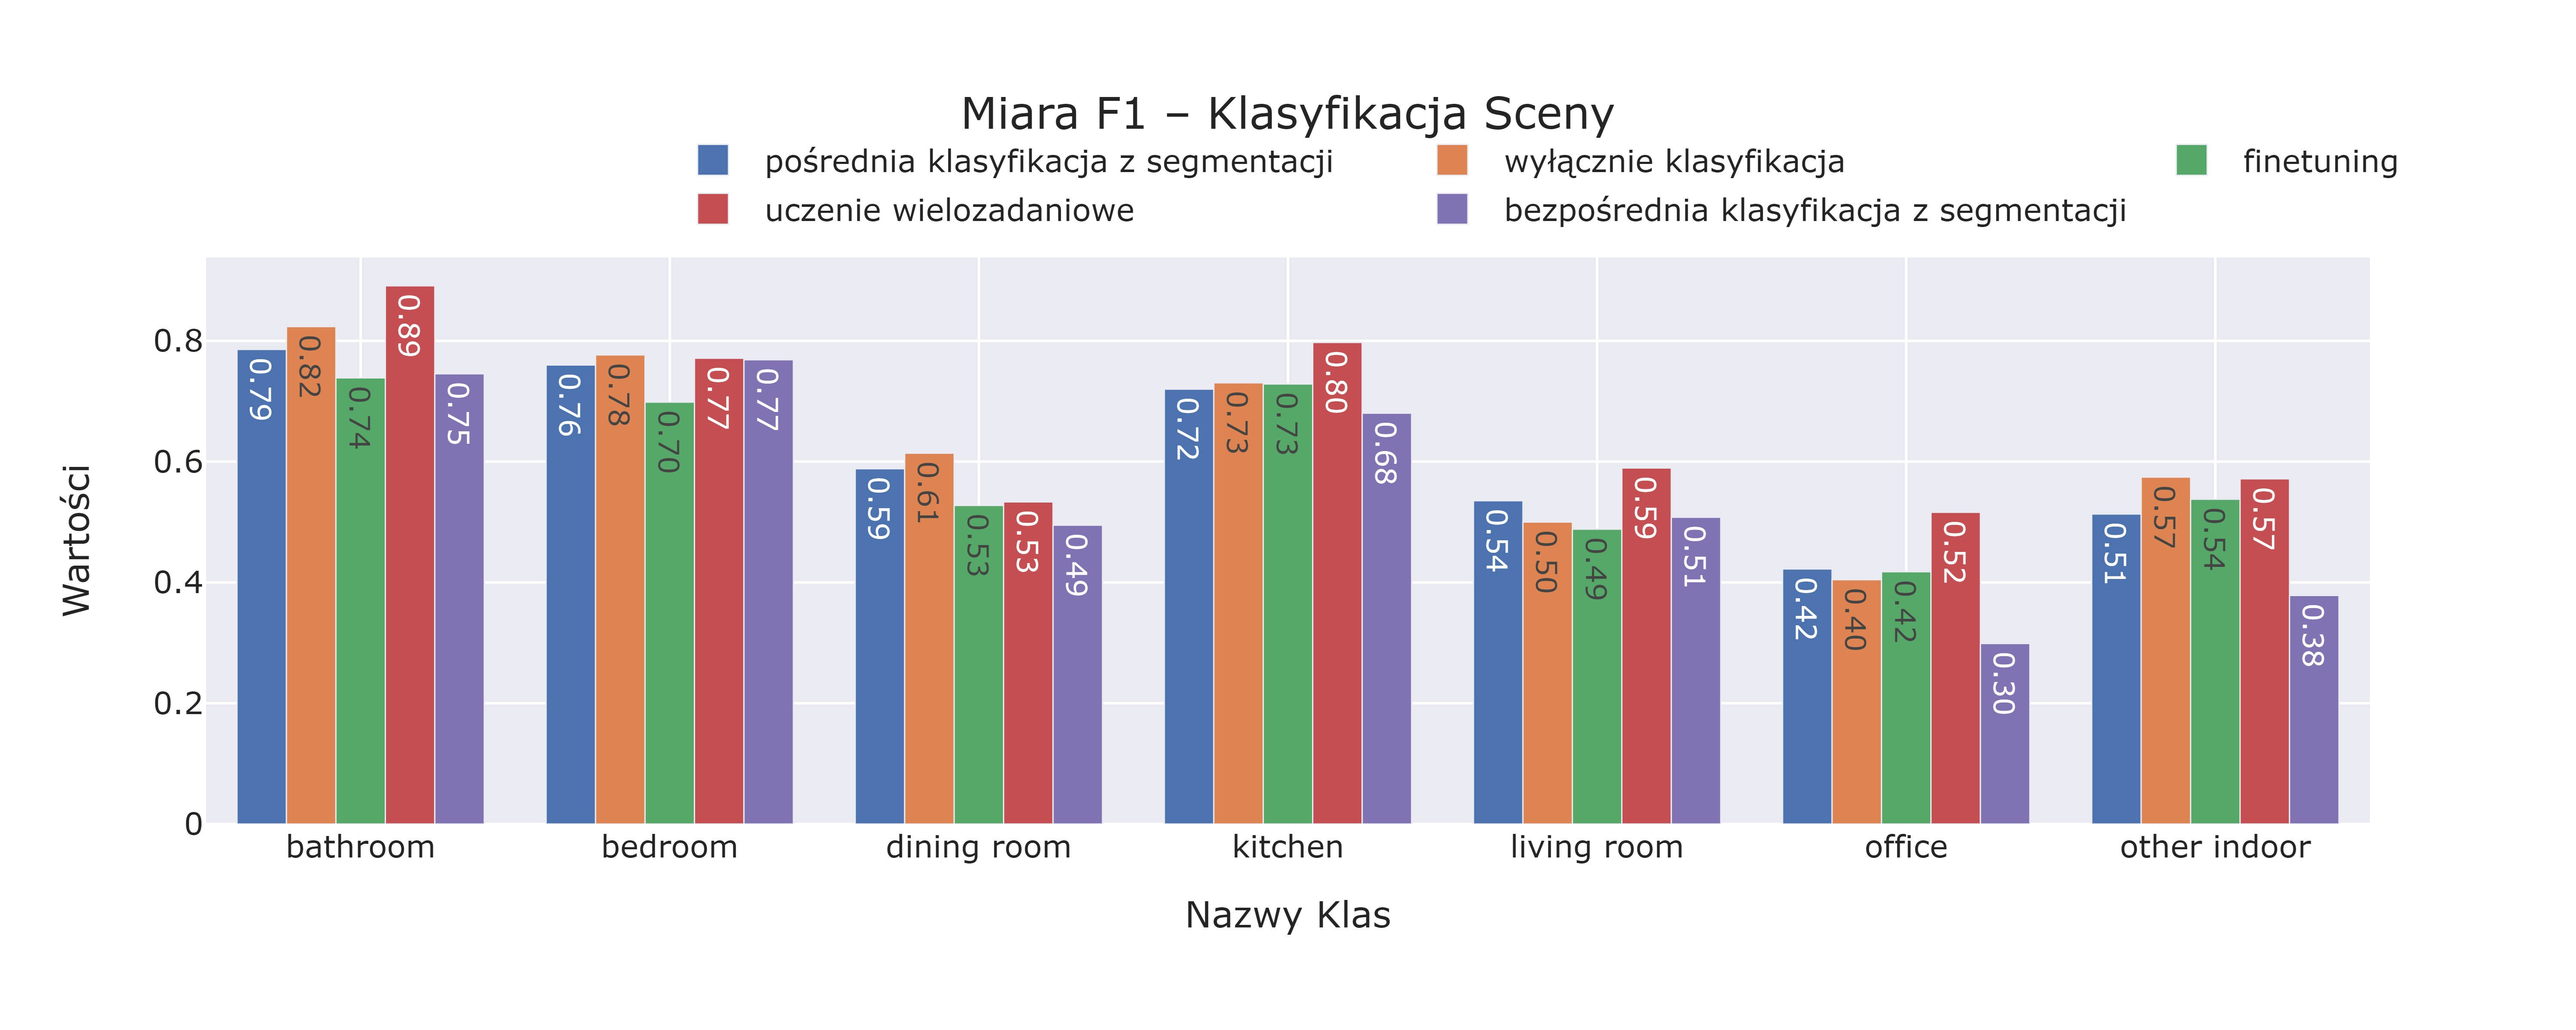
\includegraphics[width=\textwidth]{images/pl-res/Miara-F1-Klasyfikacja-Sceny.jpeg}
        \caption{Porównanie miary F1 dla klasyfikacji sceny z rozróżniem konkretnych klas.}
        \label{fig:classification-f1}
    \end{figure}
\end{frame}

\begin{frame}{Miary jakości segmentacji}
    
    \begin{figure}[ht!]
        \centering
        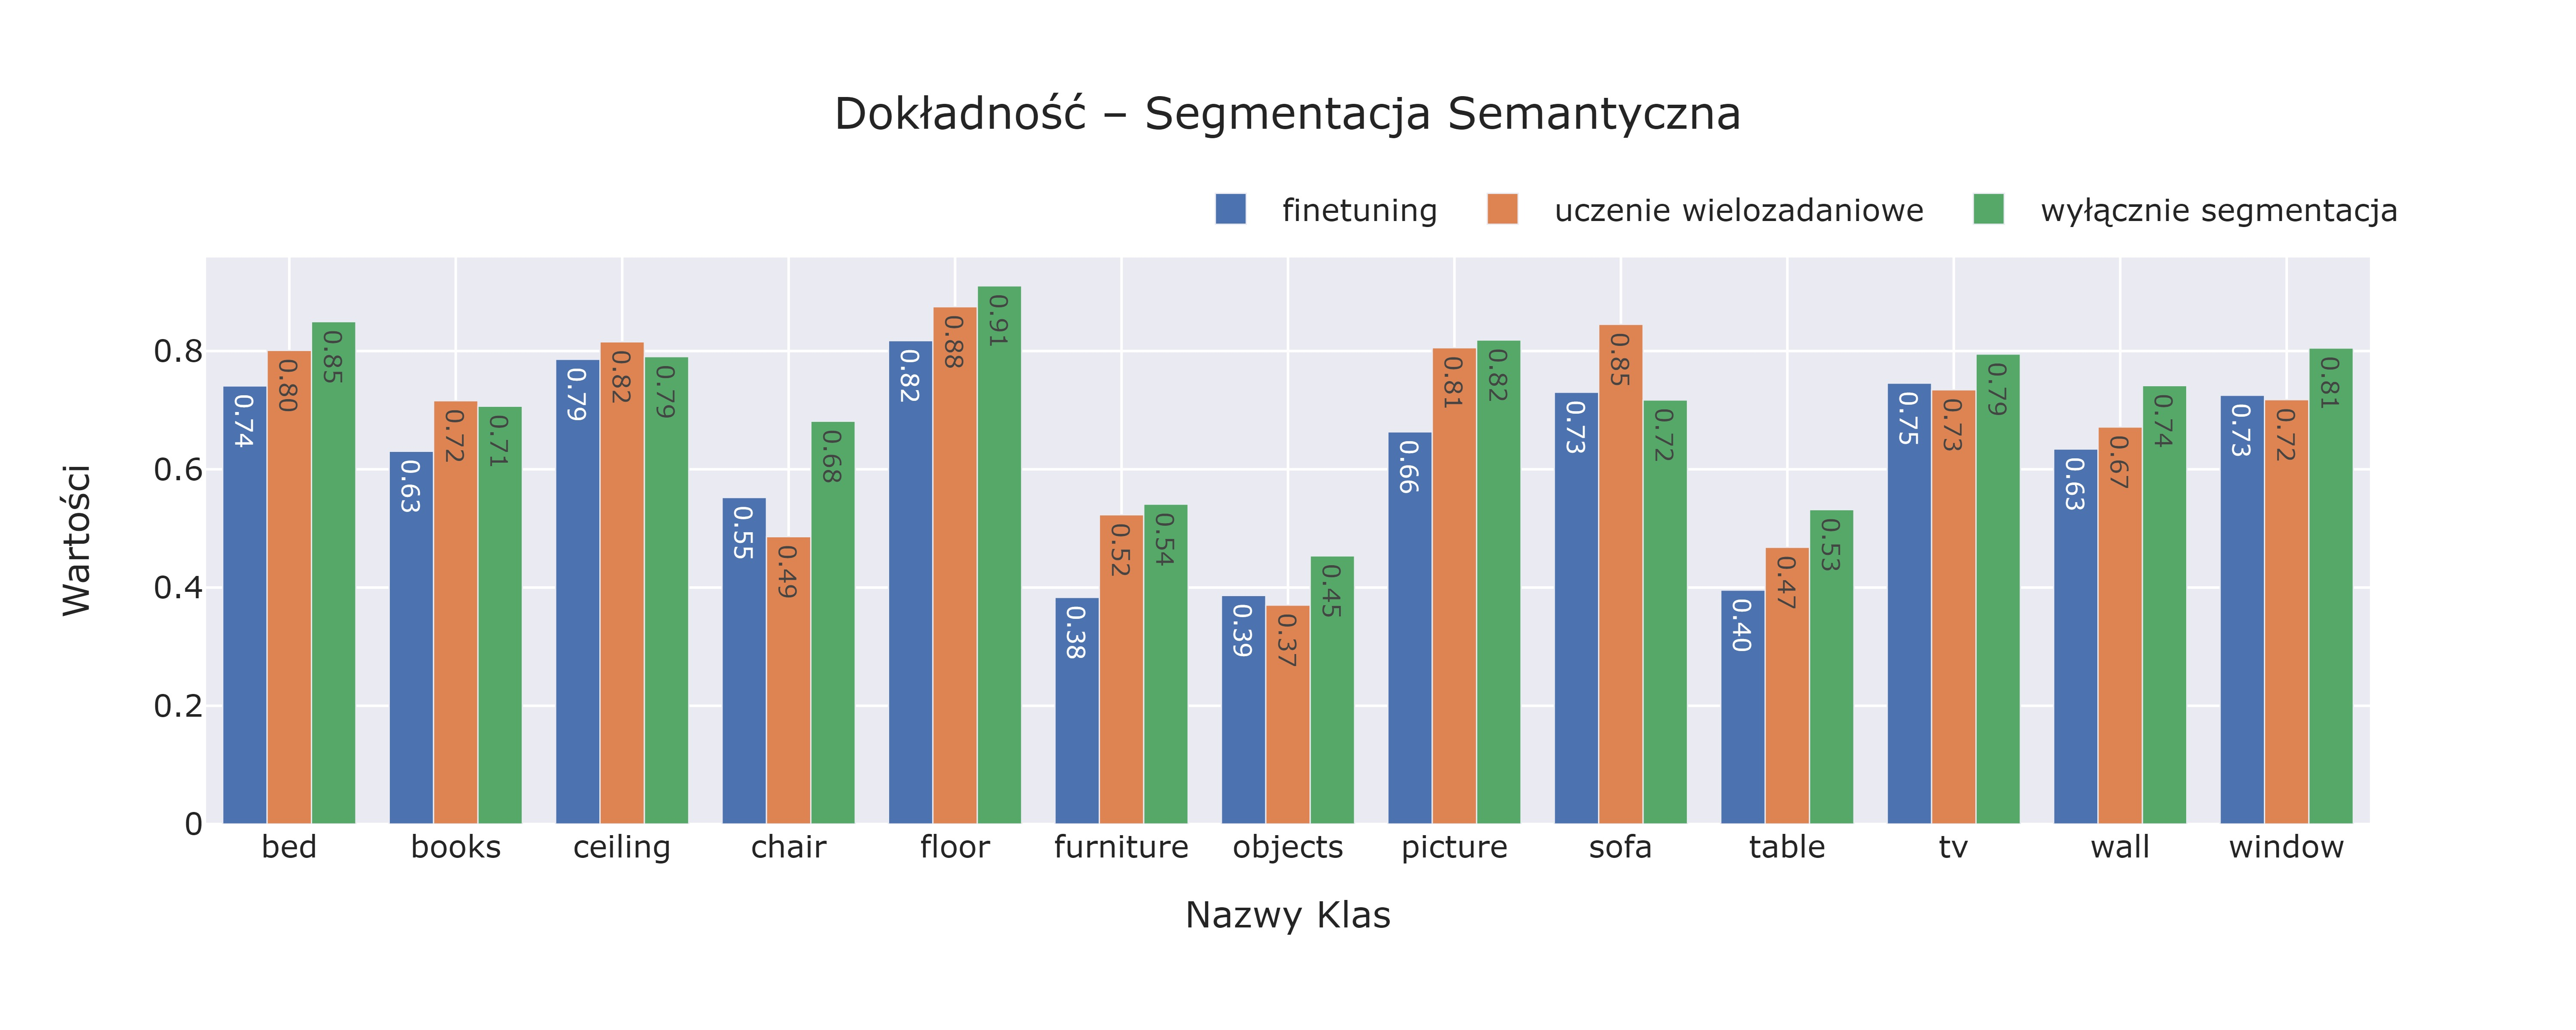
\includegraphics[width=\textwidth]{images/pl-res/Dokladnosc-Segmentacja-Semantyczna.jpeg}
        \caption{Porównanie dokładności segmentacji z rozróżniem konkretnych klas.}
        \label{fig:segmentation-acc}
    \end{figure}
\end{frame}


\begin{frame}{Miary jakości segmentacji}
    
    \begin{figure}[ht!]
        \centering
        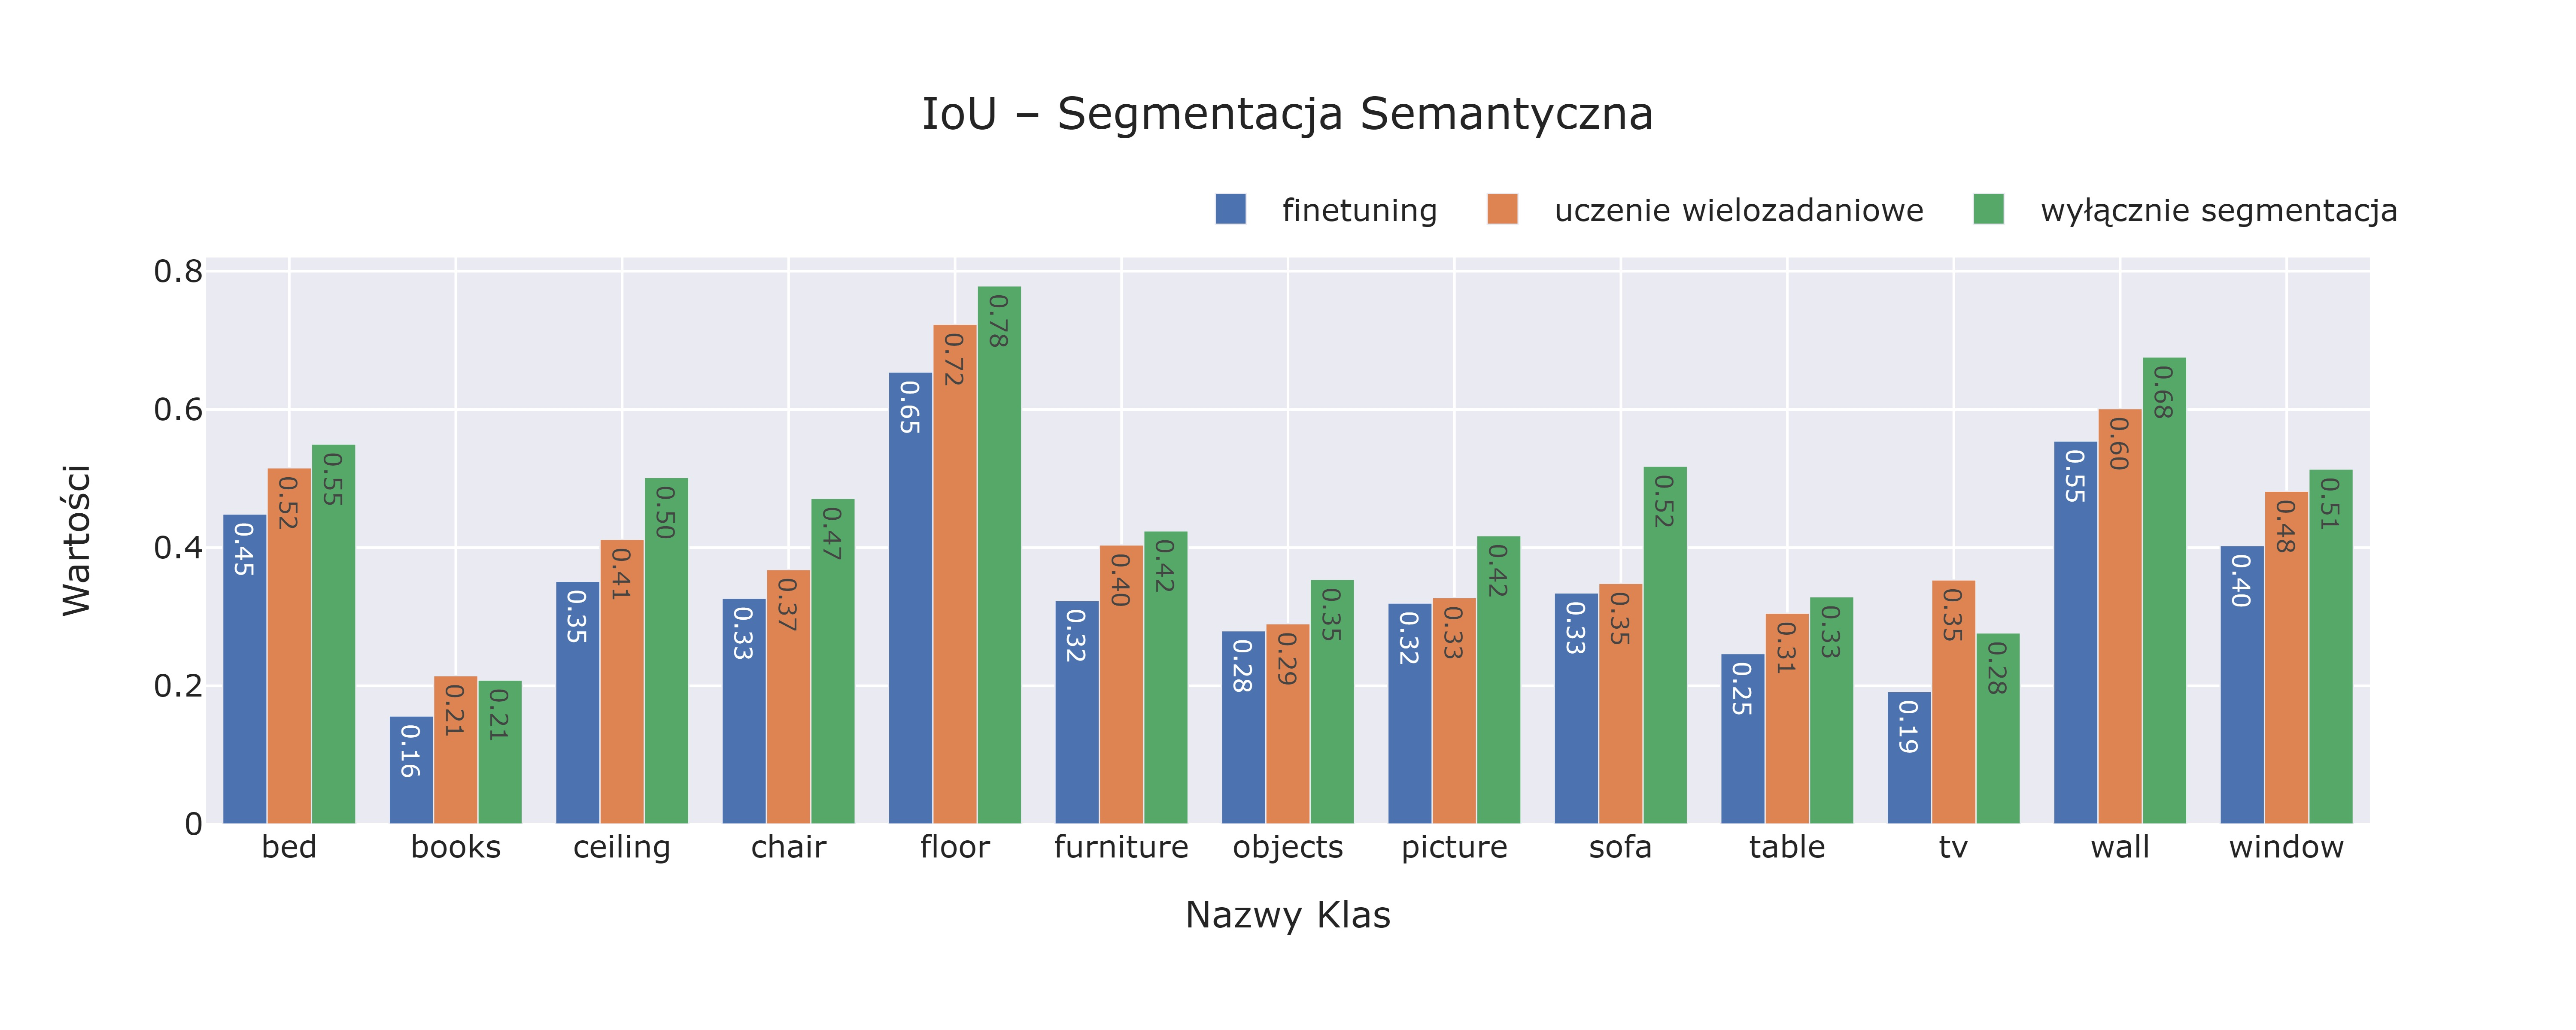
\includegraphics[width=\textwidth]{images/pl-res/IoU-Segmentacja-Semantyczna.jpeg}
        \caption{Porównanie miary IoU segmentacji z rozróżniem konkretnych klas.}
        \label{fig:segmentation-iou}
        
    \end{figure}
\end{frame}








\end{document}






